\documentclass[spanish,a4paper,11pt]{article}
\usepackage{graphicx}
\usepackage{float}
\usepackage[export]{adjustbox}
\usepackage[affil-it]{authblk}
\usepackage[utf8]{inputenc}
\usepackage[spanish]{babel}
\usepackage{booktabs}
\usepackage{multirow}
\usepackage{siunitx}
\setlength{\parskip}{2mm} % {6mm}
\usepackage{derivative}
\usepackage[margin=2.5cm]{geometry}
\usepackage{amsmath}
\usepackage{amssymb}
\usepackage{svg}
\usepackage[font={footnotesize}, labelfont=bf]{caption}
\usepackage{subcaption}
\usepackage{chngcntr}
\makeatletter
\newcommand*{\centerfloat}{%
	\parindent \z@
	\leftskip \z@ \@plus 1fil \@minus \textwidth
	\rightskip\leftskip
	\parfillskip \z@skip}
\makeatother
\counterwithin{figure}{section}
\counterwithin{table}{section}
\counterwithin{equation}{section}

\usepackage{geometry}
\usepackage{fancyhdr}
\usepackage[dvipsnames]{xcolor}
\usepackage{appendix}
\usepackage{multirow}
\usepackage{longtable}
\usepackage[font=footnotesize, labelfont=bf, width=0.8\textwidth, justification=justified]{caption}
\usepackage[pdfencoding=auto, psdextra]{hyperref}
\usepackage{titlesec}
\usepackage{csquotes}
\usepackage[backend=biber, sorting=none]{biblatex}
\usepackage{listings}

\definecolor{codegreen}{rgb}{0,0.6,0}
\definecolor{codegray}{rgb}{0.5,0.5,0.5}
\definecolor{codepurple}{rgb}{0.58,0,0.82}
\definecolor{backcolour}{rgb}{0.95,0.95,0.92}

\lstdefinestyle{mystyle}{
	backgroundcolor=\color{backcolour},   
	commentstyle=\color{codegreen},
	keywordstyle=\color{magenta},
	numberstyle=\tiny\color{codegray},
	stringstyle=\color{codepurple},
	basicstyle=\ttfamily\footnotesize,
	breakatwhitespace=false,         
	breaklines=true,                 
	captionpos=b,                    
	keepspaces=true,                 
	numbers=left,                    
	numbersep=5pt,                  
	showspaces=false,                
	showstringspaces=false,
	showtabs=false,                  
	tabsize=2,
	literate={á}{{\'a}}1 {é}{{\'e}}1 {í}{{\'i}}1 {ó}{{\'o}}1 {ú}{{\'u}}1 {Ñ}{{\~N}}1 {ñ}{{\~n}}1
}

\lstset{style=mystyle}
\addbibresource{bibliografia.bib}
\pagestyle{fancy}
\fancyhf{} % Limpia todos los encabezados y pies de página
% Redefinimos el formato para que diga "1. Nombre de la sección" (sin mayúsculas forzadas)
\renewcommand{\sectionmark}[1]{\markboth{\thesection.\ #1}{}}
\lhead{\leftmark} % Imprime dinámicamente el nombre de la sección a la izquierda
\rfoot{\thepage} % Número de página abajo a la derecha
\renewcommand{\headrulewidth}{0.4pt} % Asegura la línea horizontal debajo del encabezado

\begin{document}
	\renewcommand{\listtablename}{Índice de tablas}
	\renewcommand{\tablename}{Tabla}
	
	% ==========================================
	% CARÁTULA ESTILO FCEN
	% ==========================================
	\begin{titlepage}
		\centering
		
		% 1. Título principal arriba y en negrita
		\vspace*{0.8cm}
		{\LARGE \textbf{Asimetrías Azimutales de la Densidad de Muones en Lluvias Atmosféricas Extensas con el Detector Subterráneo de Muones del Observatorio Pierre Auger}\par}
		
		% 2. Tipo de documento
		\vspace{1.5cm}
		{\Large Tesis de Licenciatura en Ciencias Físicas\par}
		
		% 3. Autor
		\vspace{1.5cm}
		{\Large Lautaro Silva Pizzi\par}
		
		% 4. Directores y Lugar de trabajo
		\vspace{2cm}
		{\large	\textbf{Directores:} Dr. Juan Manuel Figueira y Dr. Federico Sánchez \\
			[0.5cm] Instituto de Tecnologías en Detección y Astropartículas (ITeDA) - CNEA \par}
		
		% 5. Logos (Ajustar nombres de archivos y tamaño según necesites)
		\vspace{1.5cm}
		\begin{figure}[H]
			\centering
			
\includegraphics[height=4.5cm]{imagenes/UBA.png} \hspace{2cm} % Logo UBA
			
\includegraphics[height=4.5cm]{imagenes/logo-portada5-iteda.png}  % Logo ITeDA
		\end{figure}
		
		% 6. Jerarquía institucional y fecha abajo de todo
		\vfill
		{\large 
			Departamento de Física \\
			Facultad de Ciencias Exactas y Naturales \\
			Universidad de Buenos Aires \\[0.5cm]
			Buenos Aires, Argentina \\
			Agosto 2026 \par}
		
	\end{titlepage}
	
	% ==========================================
	% RESUMEN (Página independiente)
	% ==========================================
	\newpage
	\thispagestyle{empty}
	\vspace*{2cm}
	\begin{center}
		\Large \textbf{Resumen}
	\end{center}
	\vspace{1cm}
	Aquí va el resumen detallando el hallazgo del Sweet Spot en $\theta \approx 40^\circ - 55^\circ$, la discrepancia MC/REC, el uso del Survival Ratio ($N_\mu^{\mathrm{UMD}} / N_\mu^{\mathrm{SD}}$), y el poder discriminatorio de masa (Protón vs. Hierro) mediante el parámetro $A_1$.
	
	\vspace{1cm}
	\noindent \textbf{Palabras clave:} Rayos Cósmicos, Observatorio Pierre Auger, UMD, Asimetría Azimutal, Composición de Masa.
	
	% ==========================================
	% AGRADECIMIENTOS (Página independiente)
	% ==========================================
	\newpage
	\thispagestyle{empty}
	\vspace*{2cm}
	\begin{center}
		\Large \textbf{Agradecimientos}
	\end{center}
	\vspace{1cm}
	Aquí van tus agradecimientos...
	
	% ==========================================
	% ÍNDICES
	% ==========================================
	\newpage
	\setcounter{page}{1} % Comienza a contar las páginas
	\tableofcontents
	\newpage
	
	% ==========================================
	% INCLUSIÓN DE SECCIONES (CAPÍTULOS)
	% ==========================================
	\section{Introducción a los Rayos Cósmicos de Ultra-Alta Energía}
\label{sec:introduccion}

\subsection{El espectro de energía y composición}
\label{subsec:espectro}

\subsection{Lluvias Atmosféricas Extensas (EAS) y el desarrollo longitudinal ($X_{max}$)}
\label{subsec:eas_xmax}

\subsection{Modelos teóricos de interacción hadrónica}
\label{subsec:modelos_hadronicos}

\subsection{Motivación y objetivos de la tesis}
\label{subsec:motivacion}

\newpage
	\section{El Observatorio Pierre Auger y la Detección Híbrida}
\label{sec:observatorio}

\subsection{Actualización AugerPrime}
\label{subsec:augerprime}

\subsection{El Detector de Superficie (SD) y sensibilidades electromagnéticas}
\label{subsec:sd}

\subsection{El Underground Muon Detector (UMD / AMIGA)}
\label{subsec:umd}
% Aquí irá el énfasis sobre el blindaje de 2.3 m de tierra y el umbral de 1 GeV.

\subsection{Geometría de las EAS y marco de referencia}
\label{subsec:geometria_eas}

\newpage
	% !TEX root = ../main.tex

\section{Fenomenología de las Asimetrías Azimutales en EAS}
\label{sec:fenomenologia}

La reconstrucción estándar de eventos se basa en el supuesto de que la densidad de partículas y especificamente de muones de una lluvia atmosférica extensa (EAS) presenta una simetría circular en el plano perpendicular a su eje de propagación en el plano de la lluvia. Sin embargo, esta hipótesis sólo es estrictamente válida para lluvias verticales. Para lluvias inclinadas, la simetría en el plano de la lluvia se rompe de manera sistemática, dando lugar a patrones en la densidad de muones que presentan una fuerte dependencia con el ángulo azimutal ($\phi$).

En este capítulo se describe el origen físico de esta asimetría, originada por la competencia entre la atenuación longitudinal de la cascada, efectos puramente cinemáticos de divergencia (geométricos) y el efecto del campo geomagnético terrestre, y se define el formalismo matemático utilizado para su parametrización armónica.

\subsection{El plano de la lluvia y la ruptura de simetría}
\label{subsec:simetria_ruptura}

Para estudiar la distribución espacial de las partículas, es imperativo distinguir entre el sistema de referencia topográfico y el sistema intrínseco de la cascada. Los detectores del Observatorio Pierre Auger se encuentran fijos sobre la superficie terrestre, definiendo el \textit{plano del suelo} (o \textit{ground plane}). Sin embargo, la física del desarrollo de la cascada posee simetría cilíndrica (en su aproximación de orden cero) respecto a su propio eje de propagación. El plano perpendicular a este eje es como se define el \textit{plano de la lluvia} (o \textit{shower plane}).

A lo largo de todo este trabajo, las coordenadas espaciales utilizadas para caracterizar la densidad de partículas —la distancia radial al núcleo ($r$) y el ángulo azimutal ($\phi$)— están estrictamente definidas sobre el plano de la lluvia. Para obtenerlas, las posiciones de las estaciones activadas en el terreno se proyectan geométricamente sobre este plano transversal al eje, tal como se esquematiza en la Figura \ref{fig:plano_lluvia}.

\begin{figure}[H]
	\centering
	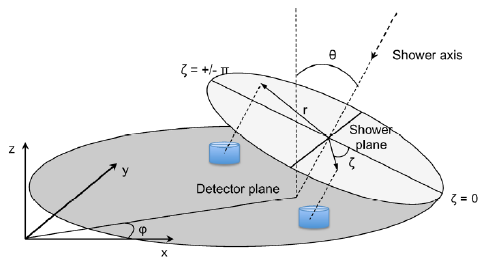
\includegraphics[width=0.7\textwidth]{capitulos/imagenes_capitulos/cap3/esquema_lluvia.png} 
	\caption{Esquema geométrico de una Lluvia Atmosférica Extensa (EAS). Se ilustra la proyección de las posiciones de los detectores desde el plano del suelo hacia el plano de la lluvia, definiendo las coordenadas intrínsecas $r$ y el ángulo azimutal $\phi$ (en el dibujo escrita como $\zeta$) del plano de la lluvia.}
	\label{fig:plano_lluvia}
\end{figure}

En el caso ideal de una lluvia estrictamente vertical ($\theta = 0^\circ$), ambos planos coinciden de manera exacta. En esta configuración, la distancia de vuelo que recorren las partículas desde el punto de primera interacción hasta alcanzar el nivel del suelo depende exclusivamente de la distancia radial al núcleo ($r$). Por lo tanto, los detectores ubicados a una misma distancia $r$ registrarán, en promedio, idénticas densidades de muones, reflejando una simetría circular perfecta e independiente del ángulo azimutal ($\phi$).


Sin embargo, cuando el rayo cósmico primario incide con un ángulo cenital $\theta > 0^\circ$, el plano de la lluvia deja de ser paralelo al plano del suelo. Esta inclinación geométrica rompe inherentemente la simetría del sistema respecto al observador terrestre.

Para comprender esta ruptura geométrica, es necesario analizar la intersección del frente plano de la lluvia con la superficie del arreglo. Al inclinar la cascada, los detectores ubicados a una misma distancia radial $r$ en el plano de la lluvia ya no se encuentran a la misma distancia física del máximo de desarrollo de la lluvia ($X_{max}$) y por ende las dinstintas particulas que componen la lluvia no atraviesan todas la misma cantidad de atomsfera antes de impactar contra el suelo. Esto define dos regiones azimutales extremas y fundamentales para el análisis de asimetrías:


\begin{itemize}
	\item \textbf{Región Temprana (\textit{Early}, $\phi \approx 0^\circ$):} Corresponde a la sección del frente de lluvia que se encuentra más cerca de la superficie topográfica y, por ende, impacta primero contra el arreglo de detectores. Las partículas que arriban a esta zona tienen el camino geométrico más corto y recorren la menor cantidad de atmósfera.
	\item \textbf{Región Tardía (\textit{Late}, $\phi \approx \pm 180^\circ$):} Corresponde a la sección diametralmente opuesta del frente, la cual se encuentra `elevada' respecto al suelo. Las partículas en esta dirección deben continuar propagándose a través de la atmósfera después de que el lado \textit{early} ya ha impactado, acumulando una distancia de vuelo significativamente mayor antes de ser detectadas y por ende siendo más atenuadas.
\end{itemize}

Esta diferencia estructural en las distancias de propagación para un mismo radio $r$ es el origen geométrico que cataliza los fenómenos físicos responsables de modular la densidad de muones, los cuales se describen a continuación.

\subsection{Origen físico de la modulación azimutal}
\label{subsec:origen_fisico}

La ruptura de la simetría circular no se debe a un único fenómeno, sino a la superposición de dos efectos principales que actúan en competencia directa y cuya dominancia depende de la distancia al eje de la lluvia.

\subsubsection{Atenuación atmosférica (dominancia \textit{early})}
\label{subsubsec:atenuacion}

El primer efecto es la atenuación atmosférica longitudinal. Las partículas que alcanzan la región tardía de la lluvia han atravesado una profundidad atmosférica considerablemente mayor que aquellas que impactan en la región temprana. Dado que la cascada evoluciona y se absorbe a medida que penetra en la atmósfera, este camino extra resulta en una mayor atenuación.

Este efecto genera un exceso aparente de densidad de partículas en la dirección $\phi = 0^\circ$ (\textit{early}) respecto a $\phi = \pm 180^\circ$ (\textit{late}). Si bien este mecanismo domina abrumadoramente la asimetría de la componente electromagnética en los detectores Cherenkov en agua (WCD), los muones, al tener un mayor poder de penetración y menor sección eficaz de interacción electromagnética, sufren una atenuación menor. No obstante, a grandes distancias del núcleo ($r > 400\text{ m}$), la atenuación atmosférica se vuelve el efecto dominante también para la componente muónica pura.

\subsubsection{Efectos geométricos y divergencia de ángulo sólido (dominancia \textit{late})}
\label{subsubsec:divergencia}

El segundo fenómeno subyacente es un efecto puramente cinemático y geométrico, producto de la divergencia de las partículas respecto al eje central de la lluvia. 

Para que una partícula alcance un detector ubicado a una distancia radial $r$ en la región temprana, debe ser emitida con un ángulo de divergencia grande respecto al eje de la cascada. Por el contrario, debido a la inclinación del frente, las partículas que impactan a la misma distancia radial $r$ en la región tardía requieren ángulos de divergencia mucho menores.

Dado que la densidad de partículas en una EAS está fuertemente concentrada cerca del eje (núcleo) y decae rápidamente conforme aumenta el ángulo de emisión, la región tardía logra muestrear una porción internamente más densa del haz primario. Este efecto geométrico induce un exceso de densidad de partículas en la región \textit{late} ($\phi = \pm 180^\circ$) que compite directamente con la atenuación atmosférica, dominando el comportamiento de la asimetría a distancias cercanas al núcleo ($r < 200\text{ m}$).

\subsection{Parametrización armónica de primer orden}
\label{subsec:parametrizacion}

Para cuantificar esta ruptura de simetría en la Función de Distribución Lateral (LDF), Billoir et al. \cite{Billoir2002} propusieron la inclusión de una parametrización de modulación cosinusoidal. Siguiendo este formalismo, la densidad de partículas (o la señal del detector) en el plano de la lluvia se modela como una función armónica de primer orden:

\begin{equation}
	S(r,\phi) = \langle S(r) \rangle \left( 1 + A_1(r, \theta) \cos\phi \right)
	\label{eq:asimetria_a1}
\end{equation}

donde $\langle S(r) \rangle$ es la densidad promedio a la distancia $r$ para una lluvia completamente simétrica, $A_1$ representa la amplitud de la asimetría temprano-tardía, y $\phi$ es el ángulo azimutal en el plano de la lluvia. Un valor de $A_1 > 0$ indica dominancia de la atenuación atmosférica (pico en la región \textit{early}), mientras que un $A_1 < 0$ señala la dominancia de efectos geométricos (pico en la región \textit{late}).

\subsection{Antecedentes en la Colaboración Auger}
\label{subsec:antecedentes}

Históricamente, el estudio de asimetrías azimutales en el Observatorio Pierre Auger se ha centrado en las señales medidas por el Detector de Superficie (SD). Los primeros estudios fenomenológicos como los de Pryke \cite{Pryke1998} y Billoir et al. \cite{Billoir2002} identificaron los patrones de asimetría en estaciones Cherenkov. Recientemente, con la actualización AugerPrime, Bradfield \cite{Bradfield2022} realizó análisis sistemáticos utilizando los detectores de superficie centelladores (SSD) combinados con los WCD, corroborando la utilidad de estas asimetrías para estudios de composición de masa.

Sin embargo, debido a que la señal del SD está invariablemente dominada por la componente electromagnética a los ángulos cenitales considerados, la magnitud intrínseca y la fenomenología de la asimetría temprano-tardía para una señal pura de muones duros ha permanecido inexplorada. Abordar este vacío utilizando las capacidades del UMD es el propósito central de los siguientes capítulos.

	\section{Simulación y Metodología de Análisis}
\label{sec:metodologia}

\subsection{Librerías Monte Carlo (CORSIKA) y reconstrucción ($\overline{\text{Offline}}$)}
\label{subsec:corsika_offline}

\subsection{Criterios de selección de eventos}
\label{subsec:cortes_seleccion}
% Cortes en energía \log_{10}(E/\mathrm{eV}) \in [17.5, 18.0]

\subsection{Estrategia del análisis azimutal: Bineado en $\sin^2\theta$}
\label{subsec:bineado_theta}

\newpage
	% !TEX root = ../main.tex

\section{Caracterización de la Asimetría en el Anillo Denso}
\label{sec:cap_anillo_denso}

En este capítulo se presentan los resultados obtenidos a partir del análisis de la asimetría azimutal en la densidad de muones utilizando la configuración de \textit{Anillo Denso}. Este marco permite estudiar la respuesta del detector y la física de la cascada en condiciones controladas, minimizando las incertidumbres vinculadas a la caída radial de la densidad de partículas. Además, este estudio permite mitigar las fluctuaciones estadísticas que podrían presentarse debido a la distribución física irregular de las estaciones en el terreno, garantizando una alta estadística por bin azimutal. Se analizan la estabilidad del parámetro $A_1$, los efectos sistemáticos de la reconstrucción y, finalmente, la capacidad de este observable para la discriminación de la masa del rayo cósmico primario.

\subsection{El Anillo Denso como entorno de control}
\label{subsec:entorno_control}

La configuración de Anillo Denso representa el escenario ideal para caracterizar la modulación azimutal. Al situar 12 estaciones virtuales a una distancia radial fija de $r = 450$~m en el plano de la lluvia, se garantiza que cualquier variación en la señal detectada sea independiente de la Función de Distribución Lateral (LDF). 

En este contexto, la densidad de partículas $S$ se modela mediante un ajuste armónico de primer orden:

\begin{equation}
	S(\phi) = \langle S \rangle (1 + A_1 \cos\phi)
	\label{eq:ajuste_armonico}
\end{equation}

donde $\phi$ es el ángulo azimutal de la estación en el plano de la lluvia, $\langle S \rangle$ es la densidad media en el anillo y $A_1$ es la amplitud de la asimetría. Como se discutió en el Capítulo 3, un valor de $A_1 > 0$ indica una dominancia del efecto de atenuación atmosférica (exceso en la zona temprana, $\phi = 0^\circ$), mientras que un $A_1 < 0$ reflejaría la dominancia de efectos geométricos y de divergencia radial (exceso en la zona tardía, $\phi = \pm 180^\circ$). 

Dado que a $r = 450$~m el sistema se encuentra fuera de la región de dominancia geométrica pura ($r < 200$~m), se espera que la contribución de los efectos de atenuación atmosférica prevalezca frente a los efectos de divergencia, permitiendo una medición estable y positiva de $A_1$.

En la Figura \ref{fig:ejemplo_ajuste} se presenta un ejemplo del ajuste realizado para una muestra de protones (modelo hadrónico \texttt{Sibyll 2.3e}) en el bin de mayor inclinación ($59.3^\circ < \theta_{\text{shower}} < 65^\circ$). Los datos corresponden a la cantidad de muones reconstruida por el UMD ($N^{\text{REC}}_\mu$). Se observan las doce estaciones virtuales equiespaciadas, donde las barras de error representan la desviación estándar estadística de la media. Se aprecia una modulación clara donde la diferencia de señal entre el máximo (región temprana) y el mínimo (región tardía) es de aproximadamente un 14\% ($\pm 7\%$ respecto a la media), confirmando una ruptura de simetría significativa para la componente muónica.

Este análisis se extendió usando también los datos de tanto la cantidad de muones inyectados por CORSIKA ($N^{\text{MC}}_\mu$) como la señal total registrada por los detectores de superficie (SD), permitiendo una comparación directa con estudios previos \cite{BradfieldThesis}. Para todos los datos se usaron las posiciones de las estaciones obtenidas a partir de la reconstrucción.

\begin{figure}[H]
	\centering
	
\includegraphics[width=1\textwidth]{capitulos/imagenes_capitulos/cap5/Ajuste_UMD_REC_Bin9.pdf}
	\caption{Ejemplo del ajuste armónico aplicado a la densidad de muones en el Anillo Denso para eventos de protón (\texttt{Sibyll 2.3e}). Los puntos representan las 12 estaciones virtuales y la curva sólida el ajuste del parámetro $A_1$ según la Ec. \ref{eq:ajuste_armonico}.}
	\label{fig:ejemplo_ajuste}
\end{figure}

 Es importante distinguir la naturaleza de los observables: mientras que el UMD cuantifica puramente la cantidad de muones, el SD registra la energía depositada total en unidades VEM (\textit{Vertical Equivalent Muon}) \cite{auger2015detector}. Esta es una unidad de energía normalizada propia del detector que considera la energía depositada de todas las partículas que atraviesan el SD, ya sean pertenecientes a la componente muónica como electromagnética de la lluvia. La evolución de $A_1$ para todos los bines cenitales se resume en la Figura \ref{fig:evolucion_asym_vs_theta}.

Al comparar las curvas, se observa que el SD presenta valores de asimetría significativamente mayores en bines de baja inclinación cenital, pero sufre un decaimiento abrupto a partir de $\theta_{\text{shower}} \gtrsim 50^\circ$. 

Este comportamiento es consistente con la fenomenología de la cascada: en lluvias más verticales, la señal del SD está dominada por la componente electromagnética (electrones y fotones), que es órdenes de magnitud más numerosa que la muónica. La discrepancia en la magnitud de la asimetría entre el SD y el UMD se fundamenta en la naturaleza de los procesos de pérdida de energía de estas partículas secundarias. La componente electromagnética está gobernada por procesos de \textit{bremsstrahlung} y creación de pares. Estos procesos están caracterizados por una longitud de radiación muy corta en la atmósfera, lo que provoca una atenuación exponencial rápida tras superar el máximo de la cascada. En contraste, los muones poseen una sección eficaz para la radiación de frenado mucho menor, dado que esta es inversamente proporcional al cuadrado de la masa. En consecuencia, pierden energía principalmente mediante ionización continua a una tasa mucho más baja y estable \cite{gaisser2016}. Esta diferencia en el poder de penetración explica por qué la amplitud $A_1$ es significativamente mayor en el SD (dominado por la atenuación abrupta de la componente EM) que en el UMD (que detecta puramente la componente muónica altamente penetrante).

\begin{figure}[H]
	\centering
	
\includegraphics[width=1\textwidth]{capitulos/imagenes_capitulos/cap5/Evolucion_Asimetria_vs_Theta.pdf}
	\caption{Evolución de la amplitud $A_1$ con su error en función de $\theta$ para el UMD (REC en azul, MC en verde) y el SD (rojo). Se observa la inversión de dominancia entre el SD y el UMD a altas inclinaciones.}
	\label{fig:evolucion_asym_vs_theta}
\end{figure}

Sin embargo, a medida que aumenta la inclinación, el espesor atmosférico recorrido crece de forma no lineal, provocando que la componente EM sea casi totalmente absorbida antes de alcanzar el nivel del suelo. En este régimen de alta inclinación, la señal del SD pasa a estar dominada exclusivamente por muones, lo que explica la caída de la asimetría medida a niveles comparables o inferiores a los del UMD. El hecho de que el $A_1$ del SD caiga incluso por debajo de los valores del UMD se atribuye a la presencia de muones de baja energía. Tal como se demuestra en el modelo de transporte cinemático \cite{Cazon2012}, estos muones de baja energía dominan a grandes distancias del núcleo y a mayores ángulos cenitales, sufriendo mayores deflexiones y retrasos geométricos. Como consecuencia, estas partículas de baja energía tienden a poblar de manera asimétrica la región tardía, lavando la asimetría de atenuación atmosférica positiva que sí logran preservar los muones más energéticos filtrados por el blindaje del UMD.

Finalmente, se observa una discrepancia sistemática entre los valores de asimetría $A_1$ obtenidos para los muones reconstruidos ($N^{\text{REC}}_\mu$) y los muones inyectados ($N^{\text{MC}}_\mu$) en el UMD. Esta diferencia, que indica un lavado o subestimación de la asimetría introducido por el framework de reconstrucción \textit{Offline}, será analizada en detalle en la sección \ref{subsec:mc_vs_rec}.

\subsection{Efectos Sistemáticos: Discrepancias MC vs. REC}
\label{subsec:mc_vs_rec}

Como se evidenció en la Figura \ref{fig:evolucion_asym_vs_theta}, existe una diferencia sistemática persistente entre la amplitud de asimetría $A_1$ obtenida a partir de muones inyectados ($N^{\text{MC}}_\mu$) y muones reconstruidos ($N^{\text{REC}}_\mu$). Dado que este análisis se realiza utilizando la geometría controlada del Anillo Denso, se descartan errores de paralaje o de reconstrucción del núcleo como fuente de la discrepancia. Por lo tanto, el origen del sesgo debe buscarse en la respuesta del algoritmo de reconstrucción del UMD o en la validez de los ajustes.

En primera instancia, se evaluó la convergencia y estabilidad de los ajustes armónicos mediante la métrica de bondad de ajuste $\chi^2_\nu$. Los resultados para todos los bines cenitales se presentan en la Figura \ref{fig:chi_cuadrado_reducido}.

Para los datos del UMD, tanto en el nivel de simulación como de reconstrucción, se obtuvieron valores de $\chi^2_\nu \approx 1$. Esto confirma que el modelo armónico de primer orden describe adecuadamente la modulación muónica y que los ajustes son estadísticamente robustos. Esto permite descartar una inestabilidad del ajuste como la fuente de la diferencia ente los valores de asimetría del UMD.

\begin{figure}[H]
	\centering
	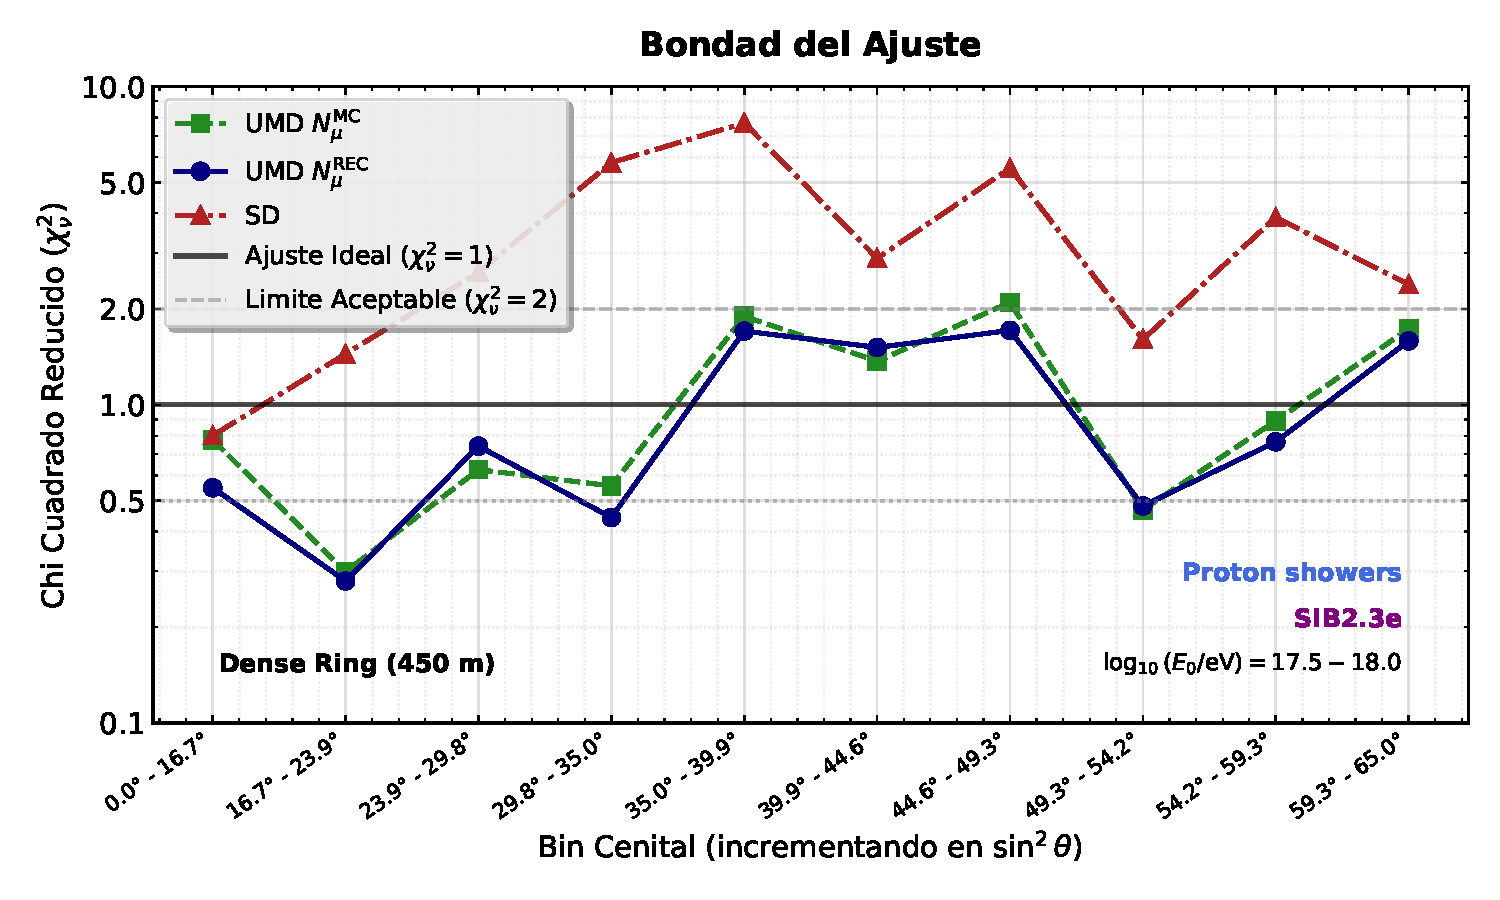
\includegraphics[width=1\textwidth]{capitulos/imagenes_capitulos/cap5/Chi2_Reduced_Fits.pdf}
	\caption{Bondad de ajuste $\chi^2_\nu$ para los bines cenitales. Se observa que los ajustes del UMD (REC y MC) se mantienen cercanos a la unidad, mientras que el SD presenta valores elevados debido a la alta precisión estadística de la muestra.}
	\label{fig:chi_cuadrado_reducido}
\end{figure}

Por el contrario, los ajustes del SD presentan valores de $\chi^2/\text{ndf}$ significativamente mayores (alcanzando un máximo de $\sim 10$). Este comportamiento no implica un fallo del modelo, sino que es consecuencia de la elevada estadística de la muestra (dado que la cantidad de partículas que llegan a los detectores es mucho mayor). Al ser el error de la media extremadamente pequeño, el test de $\chi^2$ se vuelve sensible a desviaciones de segundo orden o pequeñas asimetrías físicas que el modelo armónico simple no pretende capturar. La inspección visual del ajuste en el SD (ver Figura \ref{fig:anexo_ajuste_sd_bin9} en el Anexo \ref{anexo:ajustes_anillo_denso}) confirma que la curva describe la tendencia general de los datos con precisión, pero la rigurosidad estadística del $\chi^2$ penaliza los residuos mínimos que resultan significativos ante tan baja incertidumbre.

Para investigar la discrepancia en $A_1$ dentro del UMD, se analizó el rendimiento del algoritmo de reconstrucción de muones a nivel de estación. Se definió el Residuo Relativo de Muones como:

\begin{equation}
	\text{Residuo Relativo} = \frac{N^{\text{REC}}_\mu - N^{\text{MC}}_\mu}{N^{\text{MC}}_\mu}
\end{equation}

Esta métrica permite cuantificar el sesgo en el conteo de partículas de manera normalizada. La distribución de este residuo para la muestra de protones (\texttt{Sibyll 2.3e}) se muestra en la Figura \ref{fig:bias_umd_global}.

Si bien la distribución está centrada cerca del cero con una resolución aceptable, presenta una asimetría marcada respecto del cero. Mientras que el error por sub-reconstrucción está limitado físicamente (el residuo no puede ser menor a -1), el algoritmo presenta una cola de sobre-reconstrucción donde el número de muones detectados puede superar ampliamente al inyectado. Este fenómeno de 'sobreconteo' es intrínseco a los algoritmos de reconstrucción.

\begin{figure}[H]
	\centering
	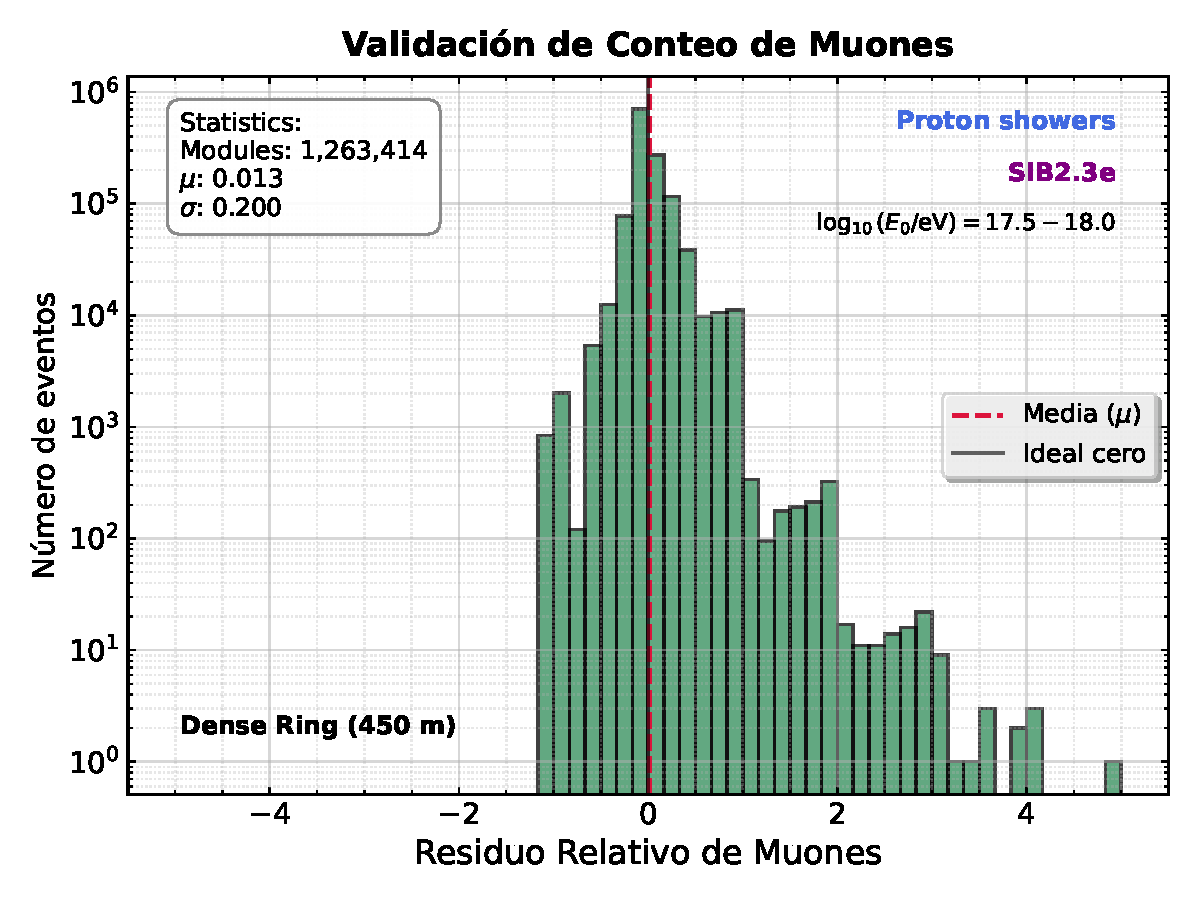
\includegraphics[width=1\textwidth]{capitulos/imagenes_capitulos/cap5/muon_counting_validation.pdf}
	\caption{Distribución del residuo relativo en la reconstrucción de muones. Aunque la media es cercana a cero, se observa una asimetría intrínseca con una cola extendida hacia la sobre-reconstrucción de partículas.}
	\label{fig:bias_umd_global}
\end{figure}

Se intento ver si esta asimetría de la distribución respecto del cero podía explicar las diferencias de la amplitud de asimetría $A_1$ entre los datos REC y los datos MC. Para esto se construyo un modelo que implementase la distribución encontrada en la Figura \ref{fig:bias_umd_global} en los datos. Sin embargo, este procedimiento solo inyectó ruido estadístico en los ajustes, sin lograr desplazar los valores de $A_1^{\text{MC}}$ hacia los niveles de $A_1^{\text{REC}}$. Este resultado negativo sugiere que el sesgo de reconstrucción no es uniforme, sino que posee una dependencia funcional con, por ejemplo, la posición de la estación o la densidad local de partículas.

\subsubsection{Bias Direccional en la Reconstrucción}
\label{subsec:bias_direccional}

Se planteó la hipótesis de que el error de conteo del UMD no es uniforme, sino que presenta una dependencia con la región azimutal de la lluvia. Si el sobreconteo es proporcionalmente mayor en las zonas de baja densidad ($\phi \approx \pm 180^\circ$) que en las de alta densidad ($\phi \approx 0^\circ$), el efecto resultante sería un aumento artificial del 'piso' de la señal tardía. Esto reduciría la modulación relativa entre ambas regiones, resultando en una degradación sistemática de la amplitud $A_1$ reconstruida.

Para verificar esta premisa, se estudió la evolución del valor medio del residuo relativo para lluvias inclinadas ($40^\circ \le \theta_{\text{shower}} \le 65^\circ$) particionando la muestra en 12 bines azimutales equiespaciados en el plano de la lluvia. Los resultados se presentan en la Figura \ref{fig:bias_direccional_rec}.

\begin{figure}[H]
	\centering
	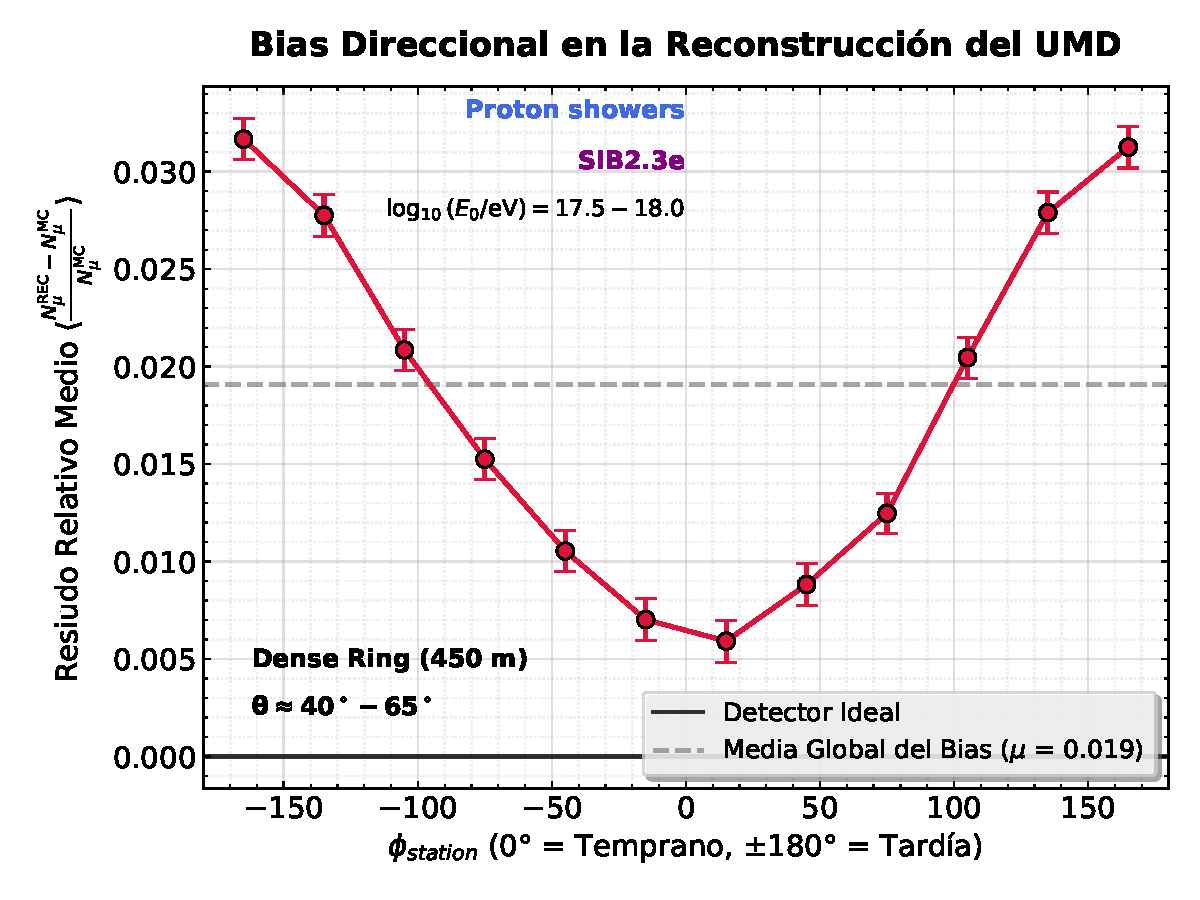
\includegraphics[width=1\textwidth]{capitulos/imagenes_capitulos/cap5/directional_bias.pdf}
	\caption{Distribución de la media del residuo relativo de reconstrucción en función del ángulo azimutal de la estación en el plano de la lluvia. Se evidencia un desempeño degradado en las regiones tardías ($\pm 180^\circ$), donde el sesgo de sobreconteo es máximamente superior al de la región temprana ($0^\circ$).}
	\label{fig:bias_direccional_rec}
\end{figure}
	
Como se observa, el algoritmo de reconstrucción presenta un sesgo positivo significativamente mayor en las regiones tardías. Físicamente, esto se debe a que en las zonas de menor densidad, cualquier fluctuación estadística o error en la deconvolución de trazas tiene un impacto relativo mucho mayor sobre el valor medio, elevando artificialmente la densidad de muones allí donde la atenuación atmosférica debería ser máxima. Este efecto actúa como un ruido coherente que 'lava' la asimetría física intrínseca de la cascada.

\subsubsection{Modelado del Bias: Implementación del \textit{Toy Model} empírico}
\label{subsec:toy_model}

Para caracterizar el impacto del error de reconstrucción en la amplitud medida y verificar si el sesgo direccional es suficiente para explicar la discrepancia observada entre los datos ideales y los reconstruidos, se implementó un \textit{Toy Model} de perturbación. Este modelo utiliza un enfoque de remuestreo empírico computacional, conocido como \textit{Bootstrap} \cite{efron1979bootstrap}. 

El algoritmo toma las densidades muónicas ideales ($N_{\mu}^{\text{MC}}$) en cada bin azimutal y les inyecta un factor de error extraído aleatoriamente de la distribución real de residuos relativos evaluada en la Figura \ref{fig:bias_direccional_rec} segmentados por $\phi$. Esta metodología garantiza dos condiciones físicas fundamentales: respeta estrictamente el límite de sub-reconstrucción (dado que el detector no puede reconstruir cantidades negativas de muones, el residuo empírico extraído siempre está acotado en un mínimo de $-1$), y captura con total fidelidad la cola asimétrica de sobreconteo característica del algoritmo del UMD. 

De esta manera, se evalúa la degradación resultante en $A_1$ considerando exclusivamente el efecto del ruido de conteo direccional, aislándola de otras fuentes de incertidumbre como la reconstrucción del núcleo, permitiendo su comparación directa con la asimetría reconstruida ($A_1^{\mathrm{REC}}$). Los resultados de este modelo se observan en la Figura \ref{fig:toy_model}.

\begin{figure}[H]
	\centering
	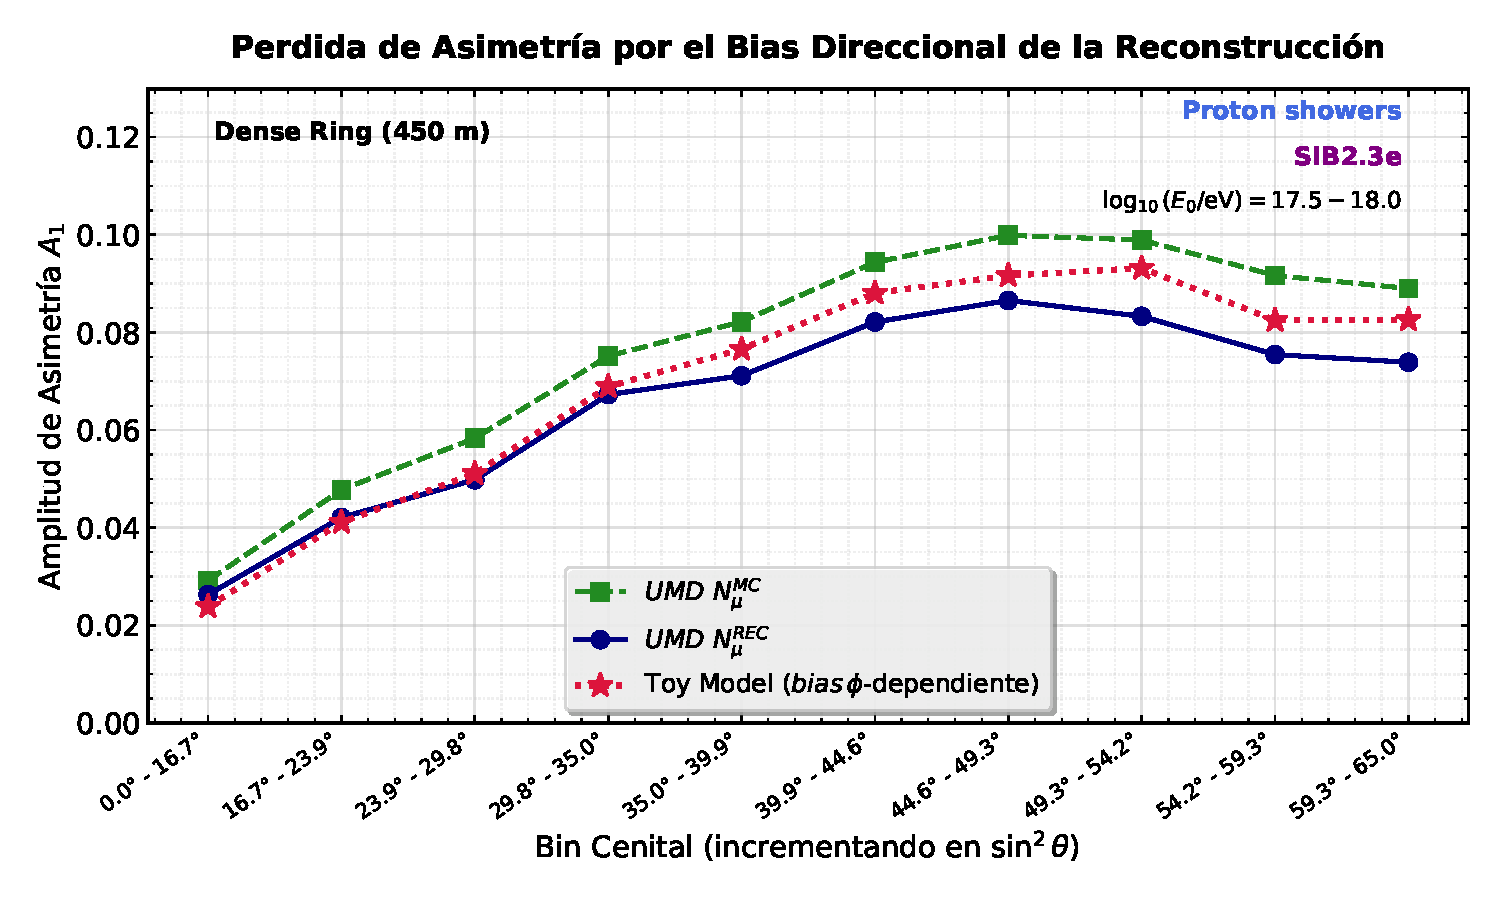
\includegraphics[width=1\textwidth]{capitulos/imagenes_capitulos/cap5/toy_model.pdf}
	\caption{Comparación de la amplitud de asimetría $A_1$ para muones inyectados (verde), reconstruidos (azul) y el resultado del \textit{Toy Model} direccional (rojo). Se aprecian dos regímenes diferenciados de degradación de señal según la inclinación de la cascada.}
	\label{fig:toy_model}
\end{figure}

El análisis de estos resultados demuestra que el \textit{Toy Model} logra reproducir el comportamiento de los datos reconstruidos, diferenciándose en dos grandes regímenes cinemáticos:

\begin{itemize}
	\item \textbf{Régimen cuasi-vertical ($\theta \lesssim 35^\circ$):} La amplitud de asimetría generada por el \textit{Toy Model} direccional se superpone casi con exactitud sobre la curva de la reconstrucción del detector ($A_1^{\mathrm{REC}}$). Esto constituye una evidencia robusta de que, en bines de baja inclinación, la totalidad de la pérdida de asimetría se origina en el sesgo de sobreconteo direccional del algoritmo de reconstrucción.
	\item \textbf{Régimen de media y alta inclinación ($\theta \gtrsim 35^\circ$):} Si bien el sesgo direccional introducido logra explicar más del 50\% de la degradación observada frente a los datos ideales, la curva del \textit{Toy Model} no alcanza a replicar la totalidad de la caída en $A_1^{\mathrm{REC}}$. Esta divergencia remanente en el régimen más inclinado indica la presencia de efectos topológicos o cinemáticos de segundo orden, tales como el \textit{lavado} azimutal introducido por la incertidumbre en la posición del núcleo o el \textit{clipping-corner}, que un modelo estadístico puramente basado en conteo unidimensional no logra capturar. 
\end{itemize}

Esta divergencia remanente señala el límite de un modelo puramente basado en la densidad de partículas. Para reproducir íntegramente la degradación de $A_1^{\mathrm{REC}}$ a altas inclinaciones, el modelo empírico debería incorporar también la incertidumbre geométrica de la reconstrucción. Como se adelantó conceptualmente en la Sección \ref{sec:procesamiento_datos}, la incerteza al ubicar la posición del impacto del núcleo reconstruido introduce un error en el cálculo del ángulo azimutal $\phi$ de cada detector en el plano de la lluvia. Considerando que la resolución típica del arreglo para la determinación del núcleo es del orden de los $20$~m, a grandes inclinaciones, debido a los efectos de compresión espacial por la proyección del frente de cascada sobre el terreno, estas variaciones generan incertezas grandes en el ángulo $\phi$ asignado a las estaciones. Este \textit{lavado} azimutal provoca que la modulación armónica se aplane aún más al mezclar cruzadamente la señal de zonas tempranas y tardías. La inyección de un ruido espacial a las coordenadas del núcleo en el \textit{Toy Model} constituiría la extensión natural para unificar y replicar los efectos instrumentales de conteo y geometría.

\subsubsection{Bias Geométrico: Absorción de la Asimetría por la LDF}

Tal como se evidenció, el sesgo de sobreconteo direccional no logra explicar la totalidad del lavado de asimetría para lluvias de alta inclinación ($\theta \gtrsim 35^\circ$) en el entorno del Anillo Denso. Esto sugiere la presencia de una segunda fuente de error sistemático. Si bien las estaciones virtuales del Anillo Denso se sitúan a un radio fijo ideal ($r = 450$~m) respecto al núcleo reconstruido, la posición absoluta de este núcleo es determinada por el algoritmo utilizando los detectores reales del arreglo (\textit{Infill}). Cualquier error sistemático en la posición de dicho núcleo afectará el cálculo angular de las estaciones virtuales que lo orbitan.

Para investigar la precisión geométrica de esta reconstrucción, se analizó el error en la determinación de la coordenada radial utilizando datos de las estaciones reales del \textit{Infill}. En la Figura \ref{fig:bias_core_azimut} se presenta el error radial ($\Delta r = r_{MC} - r_{REC}$) en función del azimutal verdadero de la estación ($\phi_{MC}$) en el plano de la lluvia. Se grafican solo las estaciones que se encuentra entre $r_{REC} \in [0,1400]m$ del eje de la lluvia.

Este gráfico revela una modulación geométrica sistemática dependiente de la región de la lluvia. En la región temprana ($\phi \approx 0^\circ$), el error es negativo ($\Delta r < 0 \implies r_{REC} > r_{MC}$), indicando que el algoritmo de reconstrucción sitúa a las estaciones artificialmente más lejos del núcleo de lo que realmente están. Inversamente, en la región tardía ($\phi \approx \pm 180^\circ$), el error es positivo, donde la reconstrucción las sitúa a las estaciones más cerca del núcleo de lo que debería. Esta deformación armónica constituye la evidencia directa de que el algoritmo de reconstrucción desplaza sistemáticamente el núcleo desde su verdadera posición hacia la región tardía de la lluvia.

\begin{figure}[H]
	\centering
	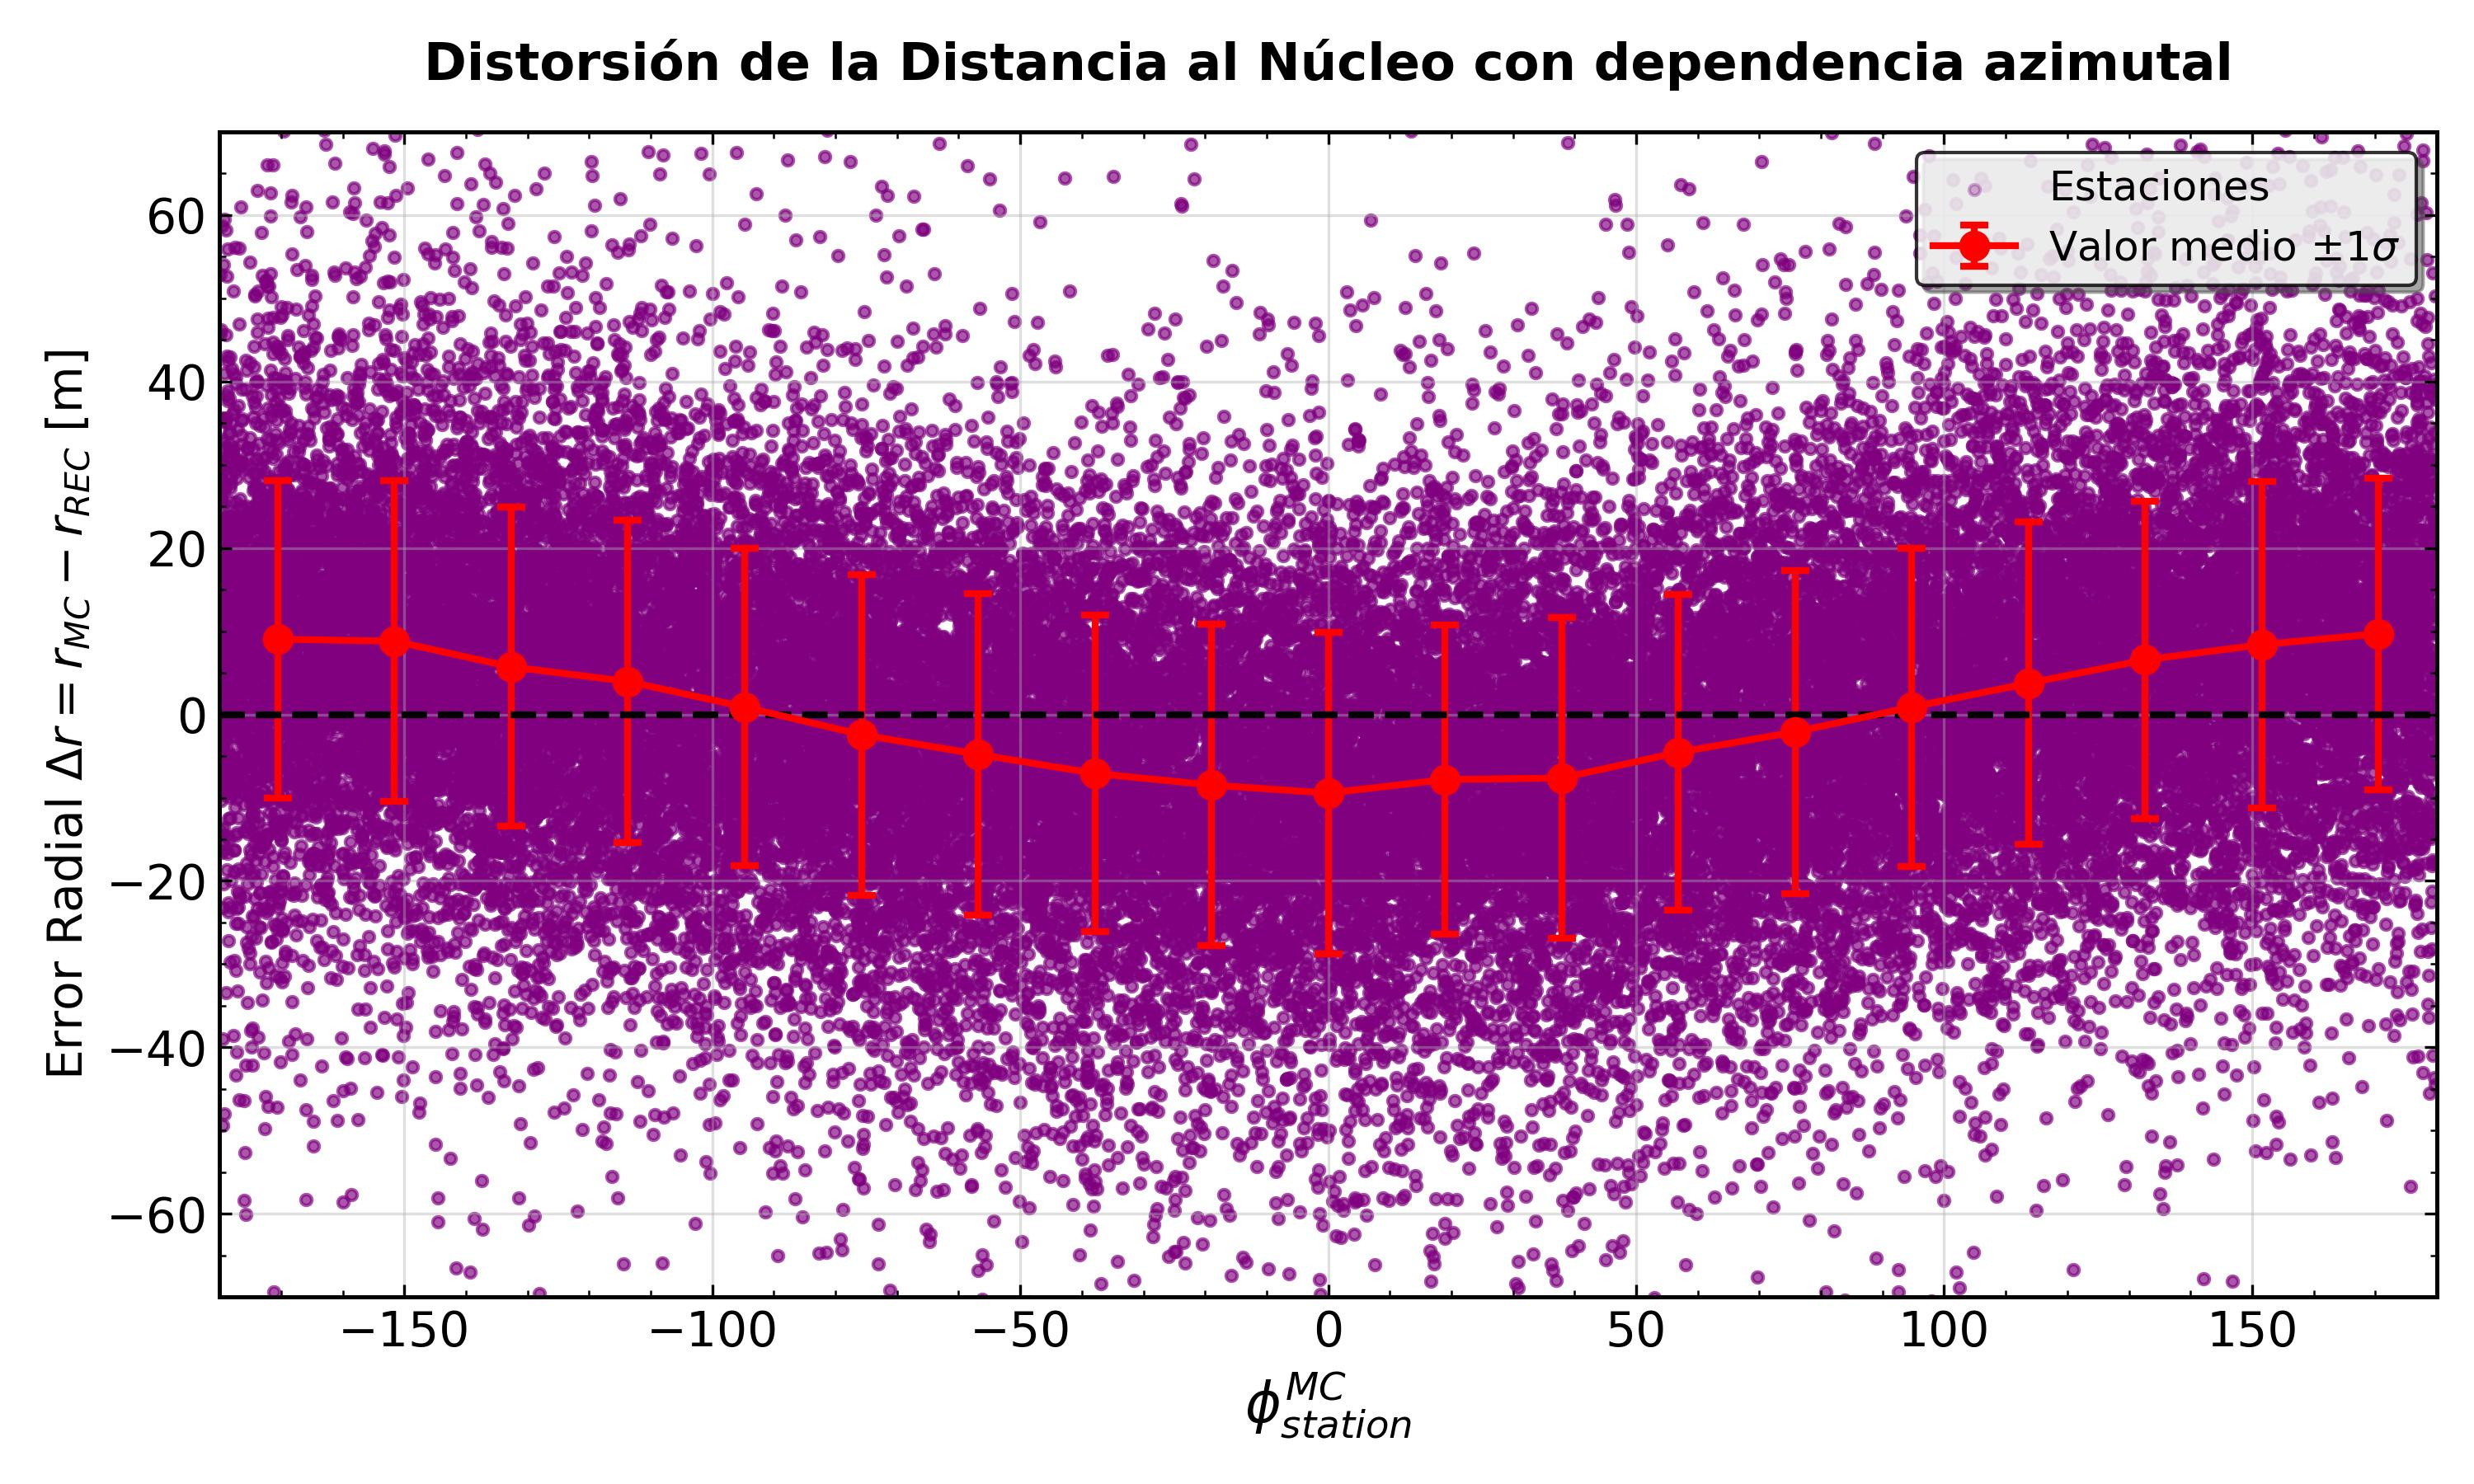
\includegraphics[width=1\textwidth]{capitulos/imagenes_capitulos/cap5/error_radial_azimut.jpg}
	\caption{Distorsión de la coordenada radial de las estaciones del \textit{Infill} en función del ángulo azimutal. La modulación armónica demuestra que el núcleo reconstruido no sufre un esparcimiento aleatorio, sino un corrimiento sistemático a lo largo del eje temprano-tardío.}
	\label{fig:bias_core_azimut}
\end{figure}

Una justificación física propuesta para explicar este comportamiento radica en la transición fenomenológica de la cascada y su conflicto intrínseco con la parametrización simétrica de la Función de Distribución Lateral (LDF). En el algoritmo de reconstrucción estándar la LDF, que se parametriza exculsivamente usando el SD, es asumida dependiente de la distancia radial pero estrictamente simétrica respecto del ángulo azimutal en el plano de la lluvia. A bajas inclinaciones, la fuerte atenuación de la abundante componente electromagnética genera asimetrías que son manejables dentro de los errores de resolución. Sin embargo, a medida que aumenta la inclinación cenital ($\theta \gtrsim 40^\circ$), la señal medida en superficie pasa a estar dominada por muones. Como se desarrollado, los muones de baja energía aumentan y se acumulan preferencialmente en la región tardía de la lluvia \cite{Cazon2012}. Esto genera una asimetría física real donde la zona tardía presenta un exceso espurio de densidad respecto a la zona temprana.

Es precisamente en este punto donde la imposición matemática del modelo simétrico falla sistemáticamente. Al intentar ajustar la posición del núcleo minimizando la función de costo, el algoritmo encuentra estaciones en la región tardía con un exceso anómalo de señal que su modelo simétrico no puede explicar si el núcleo estuviera en su posición verdadera. Dado que la LDF no contempla modulación azimutal, la única manera que tiene el ajustador para compensar esta discrepancia y lograr la convergencia es alterar la variable espacial: interpreta el exceso de señal como proximidad al eje de la cascada y la falta de señal como lejanía. Como consecuencia directa, el minimizador arrastra el núcleo reconstruido desde su posición real hacia la región tardía.

Este mecanismo explica la degradación de $A_1^{\mathrm{REC}}$ a altas inclinaciones que el \textit{Toy Model} de conteo no pudo replicar. El algoritmo \textit{Offline} impone un modelo simétrico sobre un fenómeno físicamente asimétrico (que se acentúa con el angulo cenital de la lluvia), logrando la convergencia al costo de absorber la asimetría de señal a través de un error de posición de las estaciones. Al evaluar la modulación armónica azimutal desde este núcleo reconstruido y desplazado, las estaciones tempranas quedan artificialmente más lejos de su posición relativa y las tardías artificialmente más cerca. La asimetría física es matemáticamente absorbida por el desplazamiento del núcleo, lavando la modulación azimutal y reduciendo de manera sistemática la amplitud $A_1$ observada en el UMD.

Este desplazamiento del núcleo impacta de manera crítica incluso a los datos del Anillo Denso, explicando la caída remanente del parámetro $A_1^{\mathrm{REC}}$ que el \textit{Toy Model} no pudo capturar. Aunque las estaciones del anillo virtual se sitúan a un radio de 450 m respecto al núcleo reconstruido, al estar dicho núcleo desplazado, el anillo resulta excéntrico respecto a la cascada real (MC). Esto introduce dos efectos acoplados que degradan la señal:

\begin{enumerate}
	\item \textbf{Lavado Azimutal:} Al calcular el ángulo en el plano de la lluvia desde un centro falso, el azimut asignado a cada estación difiere de su azimut físico real, mezclando de manera cruzada las señales de zonas de alta y baja densidad en el ajuste armónico.
	\item \textbf{Retroalimentación en el Conteo de Muones:} Los algoritmos del UMD que convierten las trazas de deposición de energía a número de muones reconstruidos dependen fuertemente de la geometría de incidencia de la partícula. Al suministrarse parámetros geométricos erróneos (distancias y ángulos falsos derivados del núcleo desplazado), la reconstrucción del UMD impone sesgos no lineales. Sistemáticamente se subsamplean muones en la región temprana y se sobreestiman en la tardía para forzar la compatibilidad con el modelo de LDF asimétrico, consolidando la degradación de la asimetría de atenuación original.
\end{enumerate}

En síntesis, la imposición de una LDF simétrica sobre lluvias físicamente asimétricas induce un corrimiento del núcleo que corrompe tanto la posición angular como la reconstrucción local de la señal. Esto demuestra que la asimetría física observada a nivel Monte Carlo es suprimida algorítmicamente durante la reconstrucción \textit{Offline}, lo que explica la caída de amplitud reportada a niveles de altas inclinaciones.

\subsection{Estudios de Robustez}
\label{subsec:robustez}

Se estudio también el comportamiento del detector y el parámetro de asimetría, al enfrentarse a situaciones en las que, al ser circunstancia donde la física es la misma especialmente considerando los efectos de la atenuación atmosférica, no se espera ver cambios en su performance.

\subsubsection{Invariancia azimutal de incidencia ($\phi_{shower}$)}
\label{subsubsec:invariancia_phi}

Para asegurar que la asimetría medida sea una propiedad intrínseca de la cascada y no un artefacto de la orientación del arreglo, se evaluó la estabilidad de $A_1$ en función del ángulo azimutal de entrada de la lluvia ($\phi_{\text{shower}}$). Para esto se separaron los datos del anillo denso en 6 bines equiespaciados en función del angulo de incidencia de la lluvia y se repitio el análisis explicando en la sección \ref{subsec:entorno_control} para cada uno de ellos.

 \begin{figure}[H]
	\centering
	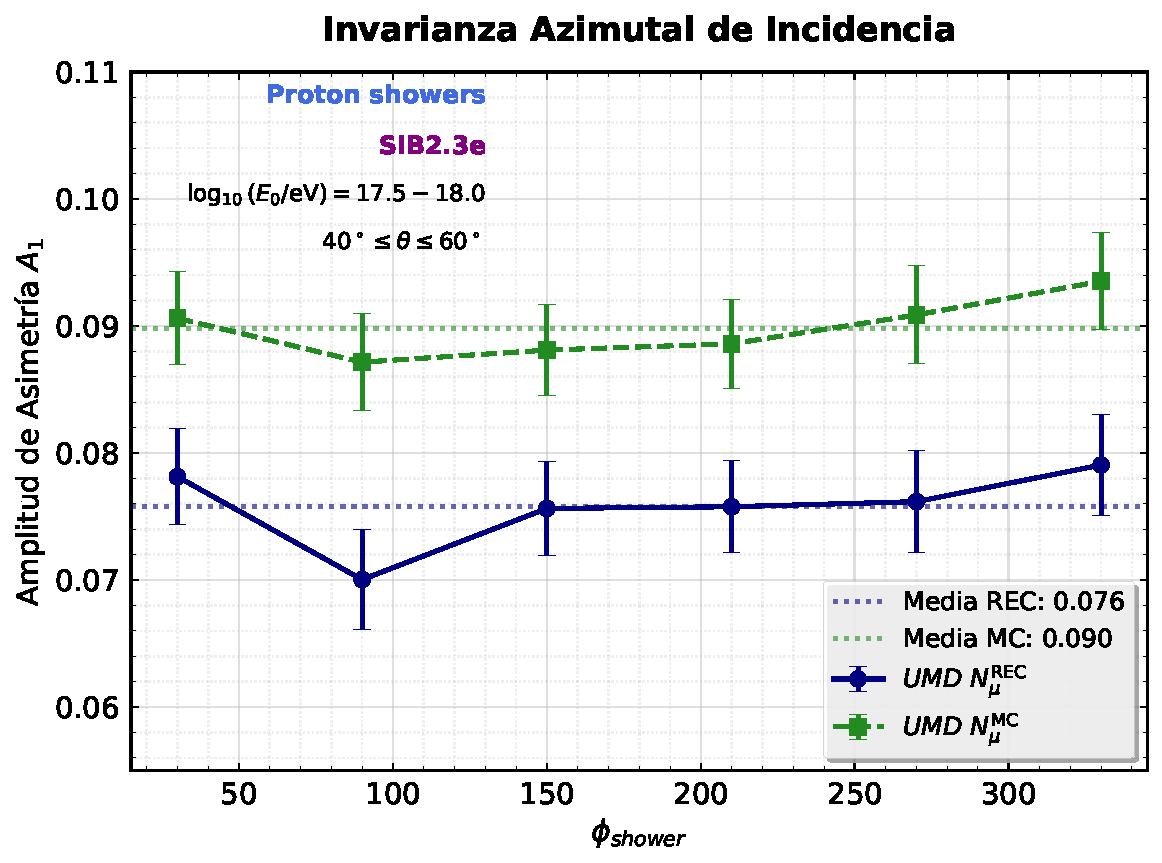
\includegraphics[width=1\textwidth]{capitulos/imagenes_capitulos/cap5/DenseRing_Systematics_Isotropy.pdf}
	\caption{Amplitud $A_1$ en función del ángulo azimutal de la lluvia. Se observa la independencia del observable respecto a la dirección de arribo.}
	\label{fig:robustez_phi}
 \end{figure}

En la Figura \ref{fig:robustez_phi} se analizo el dataset de protones con el modelo \texttt{Sibyll 2.3e} para lluvias inclinadas ($40^\circ < \theta < 60^\circ$). Se ve que el valor ajustado del parametro de asimetría $A_1$ no depende del angulo de incidencia de la lluvia, como era esperado. Esto es una buena prueba de estrés para los fundamentos del trabajo y que garantiza que se puede avanzar en el análisis en pos de hacer discriminacion de masa. Nuevamente aparece la discrepancia entre los valores absolutos de asimetria usando los muones inyectados y los reconstruidos.

\subsubsection{Independencia del modelo hadrónico}
\label{subsubsec:independencia_modelo}

Análogamente, se evaluó la robustez de la asimetría $A_1$ frente al uso de diferentes modelos de interacciones hadrónicas en las simulaciones. Para ello, se comparó la evolución del parámetro $A_1$ para un mismo primario (Helio) y rango de energía utilizando diferentes librerías fenomenológicas. Dada la disponibilidad de datos detallada en el Capítulo 4, se contrastaron las cascadas simuladas con los modelos \texttt{SIBYLL 2.3e} y \texttt{QGSJet-III.01}.

Aunque no existe garantía teórica de que ambos modelos predigan densidades totales de muones idénticas (debido a las diferencias en el déficit muónico intrínseco de cada parametrización), la modulación relativa $A_1$ debería presentar una consistencia cualitativa. Confirmar esta independencia es fundamental para validar el uso de la asimetría en la discriminación de masa y justificar la potencial combinación de conjuntos de datos para incrementar la estadística. 

Para llevar a cabo esta validación, se replicó el análisis angular realizando ajustes independientes por bin cenital, tal como se detalló en la sección \ref{subsec:entorno_control}. A su vez, se calculó la diferencia relativa porcentual entre los valores de amplitud obtenidos por ambos modelos, propagando las incertezas estadísticas correspondientes. La comparación de estas distribuciones se presenta en la Figura \ref{fig:modelos_hadronicos}.

\begin{figure}[H]
	\centering
	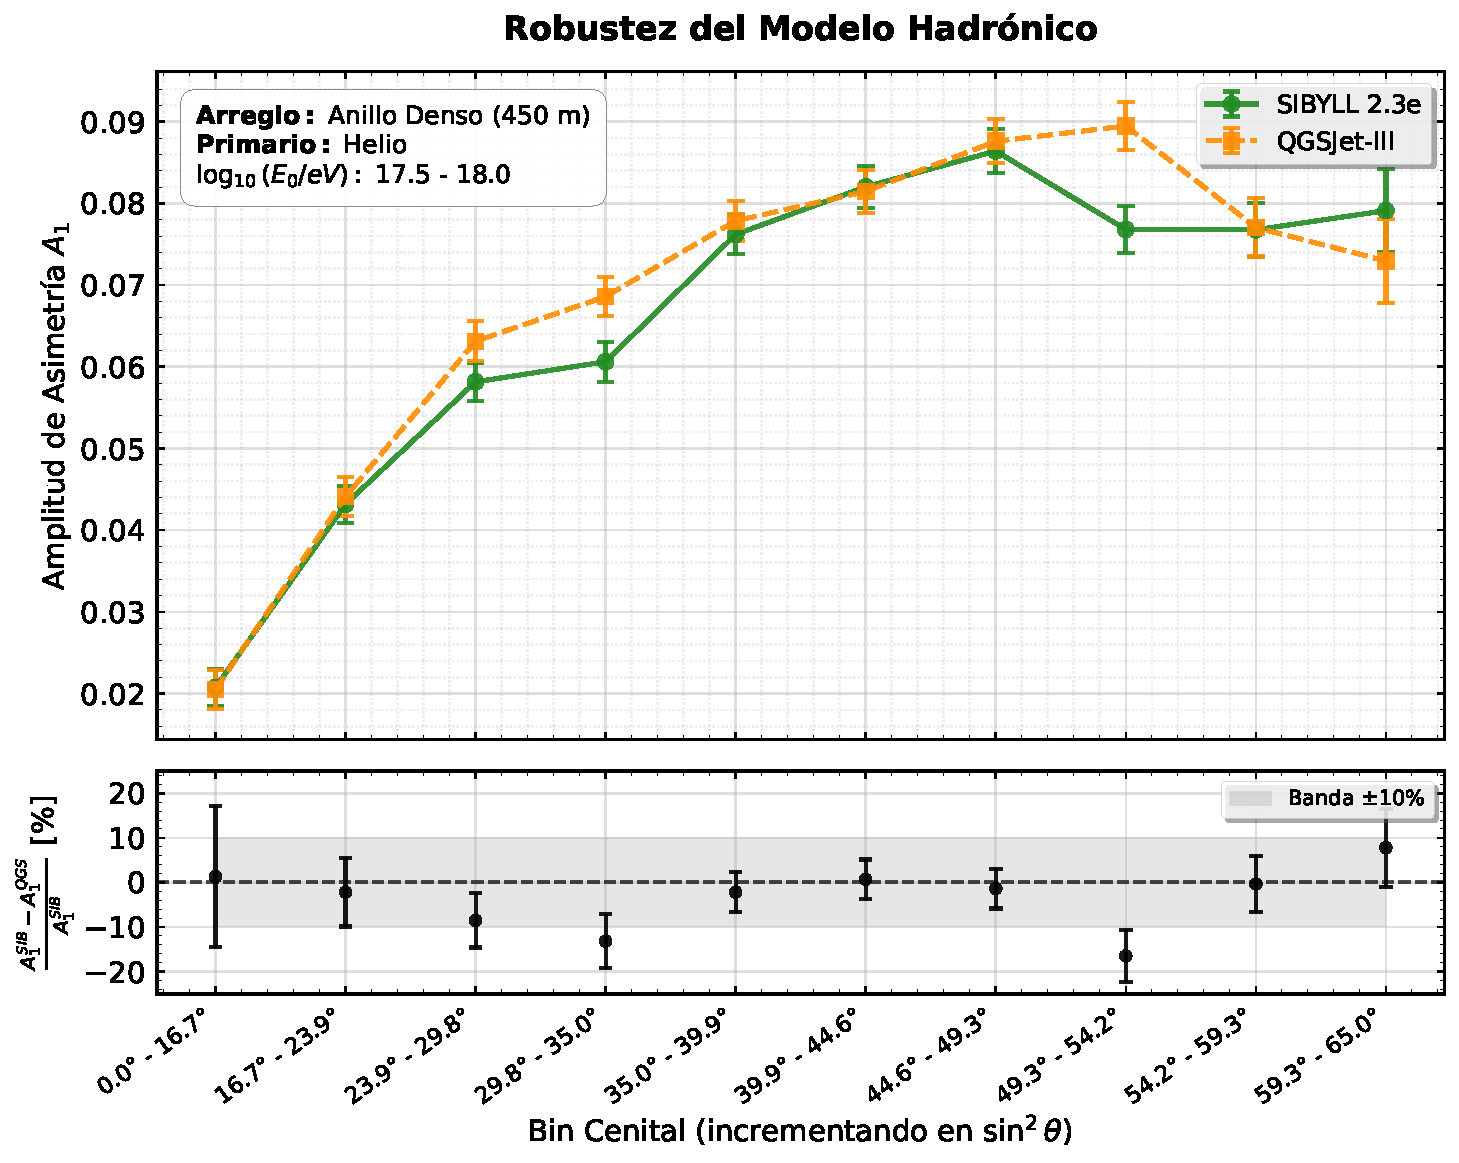
\includegraphics[width=1\textwidth]{capitulos/imagenes_capitulos/cap5/Hadronic_Uncertainty_Helium.pdf}
	\caption{Comparación de la amplitud $A_1$ para lluvias de Helio simuladas con diferentes modelos hadrónicos. El panel inferior muestra que la diferencia relativa se mantiene mayoritariamente dentro de una banda de tolerancia aceptable, indicando una tendencia común independiente del modelo.}
	\label{fig:modelos_hadronicos}
\end{figure}

Como se observa en el panel superior, la evolución de la asimetría presenta una consistencia morfológica excelente entre ambos modelos a lo largo de todo el rango angular. El panel inferior cuantifica esta concordancia: la diferencia relativa se mantiene predominantemente dentro de una banda de tolerancia del $\pm 10\%$, con desviaciones estadísticas puntuales que no superan el $15\%$. Este resultado confirma empíricamente que la amplitud de la asimetría azimutal $A_1$ es un observable robusto. Su forma funcional y magnitud relativa están dominadas por la cinemática macroscópica de la cascada y la atenuación atmosférica, manteniéndose esencialmente invariantes frente a los detalles microscópicos del modelo de interacción hadrónica empleado por el generador de Monte Carlo.

\subsection{Dependencia de la amplitud $A_1$ con la energía del primario}
\label{subsec:dependencia_energia}

Para evaluar la estabilidad del observable frente a variaciones cinemáticas, se analizó la evolución del parámetro de asimetría $A_1$ en función de la energía del rayo cósmico primario dentro de la banda de interés, $\log_{10}(E/\mathrm{eV}) \in [17.5, 18.0]$. Utilizando el conjunto de simulaciones de protones (\texttt{SIBYLL 2.3e}) restringido al rango angular de mayor desarrollo de asimetría ($40^\circ \leq \theta \leq 60^\circ$), los datos se particionaron en 5 bines de energía reconstruida. Los resultados de los ajustes armónicos para cada intervalo se presentan en la Figura \ref{fig:a1_vs_energia}.

\begin{figure}[H]
	\centering
	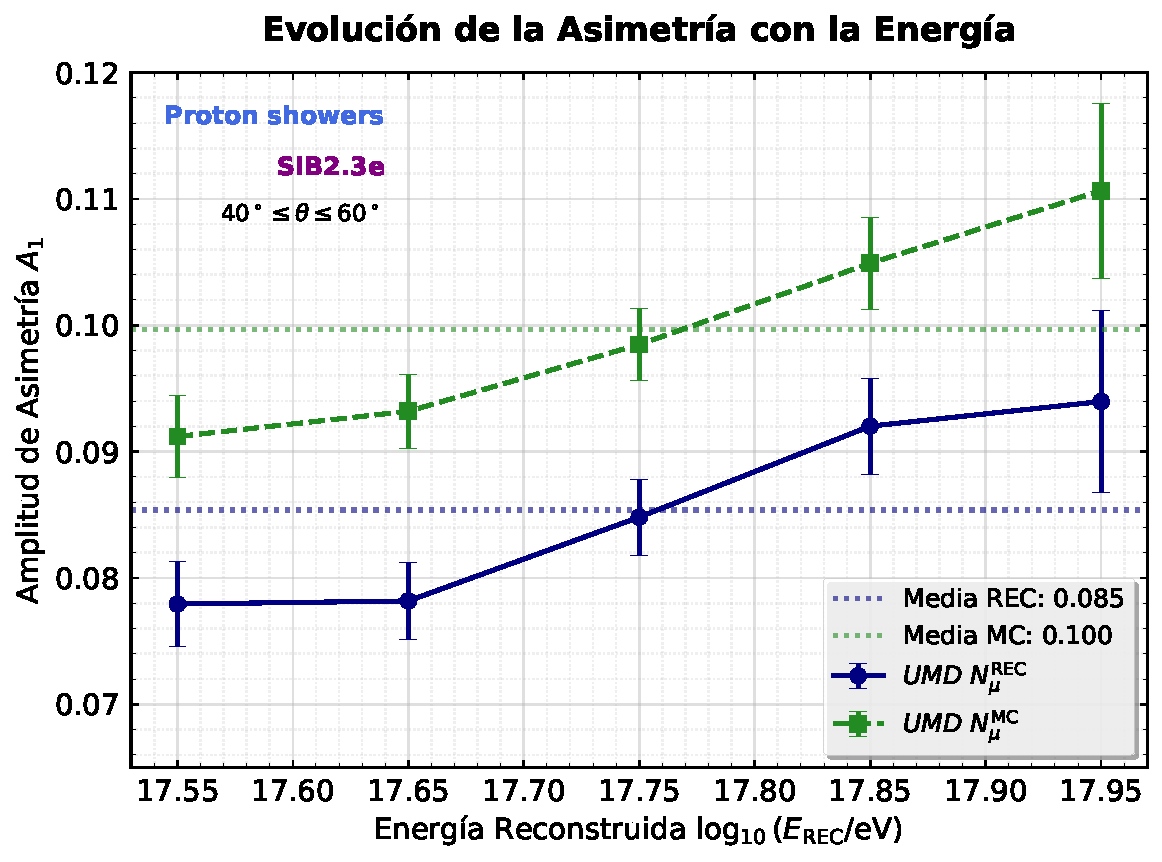
\includegraphics[width=1\textwidth]{capitulos/imagenes_capitulos/cap5/DenseRing_Systematics_Energy.pdf}
	\caption{Evolución de la amplitud de asimetría $A_1$ en función de la energía reconstruida para cascadas de protón simuladas con \texttt{SIBYLL 2.3e}. Se observa un leve incremento lineal en la asimetría a mayores energías, presente tanto a nivel Monte Carlo como en la reconstrucción.}
	\label{fig:a1_vs_energia}
\end{figure}

A priori, al tratarse de un rango energético relativamente estrecho (media década logarítmica), no se esperaba observar una fuerte dependencia funcional. Sin embargo, los resultados revelan un leve pero sistemático incremento lineal de la amplitud $A_1$ a medida que aumenta la energía, comportamiento que es capturado consistentemente tanto por los datos ideales (MC) como por los reconstruidos (REC).

La hipótesis de trabajo propuesta para explicar este comportamiento físico radica en el corrimiento de la profundidad del máximo de desarrollo de la cascada ($X_{\mathrm{max}}$). Teóricamente, un aumento en la energía del primario implica que la lluvia penetra más profundamente en la atmósfera antes de alcanzar su número máximo de partículas, acercando el $X_{\mathrm{max}}$ al nivel del suelo. Al reducirse la distancia atmosférica remanente entre el máximo de la lluvia y los detectores, la cascada observada resulta longitudinalmente más 'joven'. Esto altera los gradientes de densidad de partículas a través del plano de la lluvia, impactando directamente en la magnitud de la asimetría de atenuación. Cabe destacar que, si bien esta interpretación fenomenológica vincula lógicamente el incremento de $A_1$ con la evolución del $X_{\mathrm{max}}$, en el marco de este trabajo constituye una hipótesis interpretativa que sienta las bases para futuros estudios dedicados a correlacionar el desarrollo longitudinal con la topología en superficie.

Desde el punto de vista metodológico, el hallazgo más relevante de este escrutinio es la escala de la variación. Si bien la dependencia con la energía existe, la variación absoluta del parámetro a lo largo de toda la década es marginal ($\Delta A_1 \approx 0.015$). Esta estabilidad garantiza que la integración de todos los eventos del rango $\log_{10}(E/\mathrm{eV}) \in [17.5, 18.0]$ no inducirá un lavado ni ensanchará significativamente las distribuciones de manera crítica. Por consiguiente, queda plenamente justificado realizar el estudio de discriminación de masa primaria utilizando el \textit{dataset} completo de forma integrada, lo cual resulta imperativo para maximizar el poder estadístico sin comprometer la sensibilidad del observable.

\subsection{Discriminación de Masa Primaria: Protón vs. Hierro}
\label{sec:discriminacion_masa}

Habiendo caracterizado los efectos sistemáticos y validado la estabilidad de la reconstrucción en el entorno del Anillo Denso, el objetivo culminante de este análisis es evaluar la capacidad del observable $A_1$ para discriminar la naturaleza química del rayo cósmico primario. Para ello, se compararon las distribuciones de amplitud de asimetría para las poblaciones extremas de masa: primarios livianos (protones) y primarios pesados (hierro, conformados por 56 protones). 

Al evaluar el parámetro $A_1$ para ambos conjuntos de datos con energías $\log_{10}(E/\mathrm{eV}) \in [17.5, 18.0]$ usando el modelo hadrónico \texttt{Sibyll 2.3e}, se observó una separación sistemática entre las curvas. La población de protones desarrolla amplitudes de asimetría consistentemente mayores a las correspondientes a la población de hierro a lo largo del rango angular evaluado para la mayoría de los bines.

\subsubsection{El Factor de Mérito ($MF$) y el \textit{Sweet Spot} de discriminación}
\label{subsec:sweet_spot}

Para cuantificar rigurosamente el poder separador del observable, es necesario evaluar no solo la distancia entre los valores medios de ambas poblaciones, sino también su dispersión estadística. Con este fin, se utilizo como métrica de evaluación el Factor de Mérito ($MF$) como:

\begin{equation}
	MF = \frac{|\langle A_1^{\text{P}} \rangle - \langle A_1^{\text{Fe}} \rangle|}{\sqrt{(\sigma_{A_1}^{\text{P}})^2 + (\sigma_{A_1}^{\text{Fe}})^2}}
\end{equation}

Donde $\langle A_1 \rangle$ y $\sigma_{A_1}$ representan el valor medio y la desviación estándar de la amplitud de asimetría ajustada para cada primario. Un valor de $MF > 1$ indica un régimen donde la separación entre las distribuciones supera a sus anchos característicos, permitiendo una discriminación estadística robusta. En la Figura \ref{fig:mf_sweet_spot} se presenta la evolución del Factor de Mérito en función del ángulo cenital de la cascada.

El análisis de esta figura revela un comportamiento fuertemente dependiente de la inclinación. Se identifica de manera clara una región óptima, o \textit{Sweet Spot} de discriminación, en el rango angular $40^\circ \leq \theta \leq 55^\circ$. En esta ventana, el $MF$ alcanza valores máximos del orden de $\approx 2.5$, garantizando la excelente capacidad de la amplitud de asimetría para hacer separación de masas.

\begin{figure}[H]
	\centering
	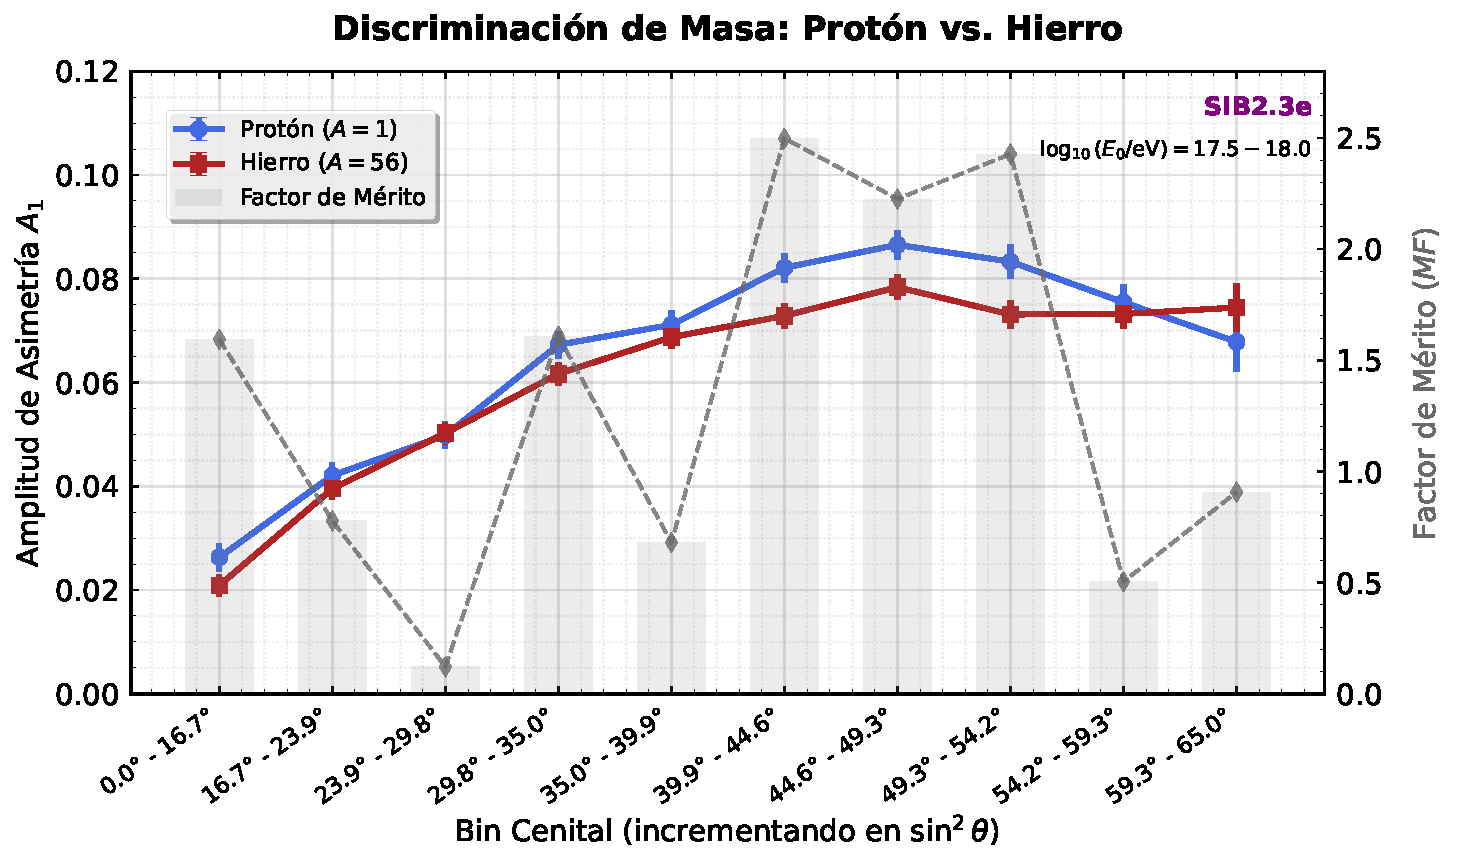
\includegraphics[width=1\textwidth]{capitulos/imagenes_capitulos/cap5/Mass_Discrimination_MF.pdf}
	\caption{Evolución del Factor de Mérito ($MF$) en función del ángulo cenital. Se identifica un \textit{Sweet Spot} de máxima separación entre bines de $40^\circ$ y $55^\circ$, donde el poder de discriminación alcanza su máximo antes de degradarse por efectos instrumentales.}
	\label{fig:mf_sweet_spot}
\end{figure}

Fuera de este rango, el poder de discriminación decae abruptamente o se vuelve inestable debido a dos regímenes limitantes de carácter completamente distinto:

\begin{enumerate}
	\item \textbf{Régimen de baja inclinación ($\theta < 35^\circ$):} En cascadas cuasi-verticales, la diferencia de camino atravesado por las partículas entre la región temprana y tardía es mínima. Por lo tanto, la asimetría de atenuación física es en modulo tan pequeña que la diferencia absoluta entre protón y hierro resulta imperceptible, quedando enmascarada por las fluctuaciones estadísticas propias de la lluvia.
	\item \textbf{Régimen de alta inclinación ($\theta > 60^\circ$):} Aunque a estos ángulos la asimetría física debería ser máxima, entra en juego el colapso de la reconstrucción instrumental. Tal como se demostró exhaustivamente en la Sección \ref{subsec:mc_vs_rec}, a grandes inclinaciones el ajustador \textit{Offline} induce un corrimiento sistemático del núcleo, entre otros problemas. Este sesgo geométrico genera un lavado azimutal y un sobreconteo direccional de muones que distorsiona la asimetría. Este efecto no solo achata artificialmente las medias de $A_1$, reduciendo el numerador del $MF$, sino que introduce un ruido correlacionado masivo que dispara el tamaño de las desviaciones estándar ($\sigma$), destruyendo por completo la capacidad discriminatoria del detector en este régimen.
\end{enumerate}

\subsection{Interpretación Física: dependencia con el $X_{max}$}
\label{subsec:interpretacion_fisica}

La existencia de una separación sistemática donde $\langle A_1^{\text{P}} \rangle > \langle A_1^{\text{Fe}} \rangle$ no es un resultado estadístico aislado, sino la manifestación en superficie de la evolución longitudinal intrínseca de la cascada atmosférica. La hipótesis de trabajo que actúa como justificación física de este fenómeno radica en la dependencia de la asimetría azimutal con la profundidad atmosférica del máximo desarrollo de la lluvia ($X_{\text{max}}$), de manera análoga al análisis realizado en la Sección \ref{subsec:dependencia_energia} respecto a la energía del primario.

Este comportamiento encuentra su marco teórico en el Modelo de Superposición y el modelo de Heitler-Matthews para cascadas hadrónicas \cite{matthews2005}. Según este esquema, una cascada iniciada por un núcleo \textbf{pesado} de masa $A$ y energía total $E_0$ se comporta estadísticamente como la superposición de $A$ sub-cascadas nucleónicas independientes, cada una portando una fracción de energía $E_0/A$. Dado que la sección eficaz de interacción crece con el tamaño del núcleo, y la energía por nucleón es sustancialmente menor, las cascadas de hierro ($A=56$) interactúan mucho más alto en la atmósfera que las de protón ($A=1$). Como resultado directo, agotan su desarrollo longitudinal prematuramente, situando el $X_{\text{max}}$ de una lluvia de hierro a una profundidad atmosférica significativamente menor (mayor altitud geográfica) comparado con las lluvias de protones. 

Esta separación en la profundidad de máximo desarrollo entre especies primarias es un fenómeno empíricamente robusto, medido de forma extensiva por los telescopios de fluorescencia del Observatorio Pierre Auger \cite{yushkov2019mass}. En la Figura \ref{fig:auger_xmax} se ilustra esta dependencia, evidenciando cómo el $X_{\text{max}}$ se ubica más profundo a mayores energías y cómo los primarios livianos penetran sistemáticamente más que los pesados.

\begin{figure}[H]
	\centering
	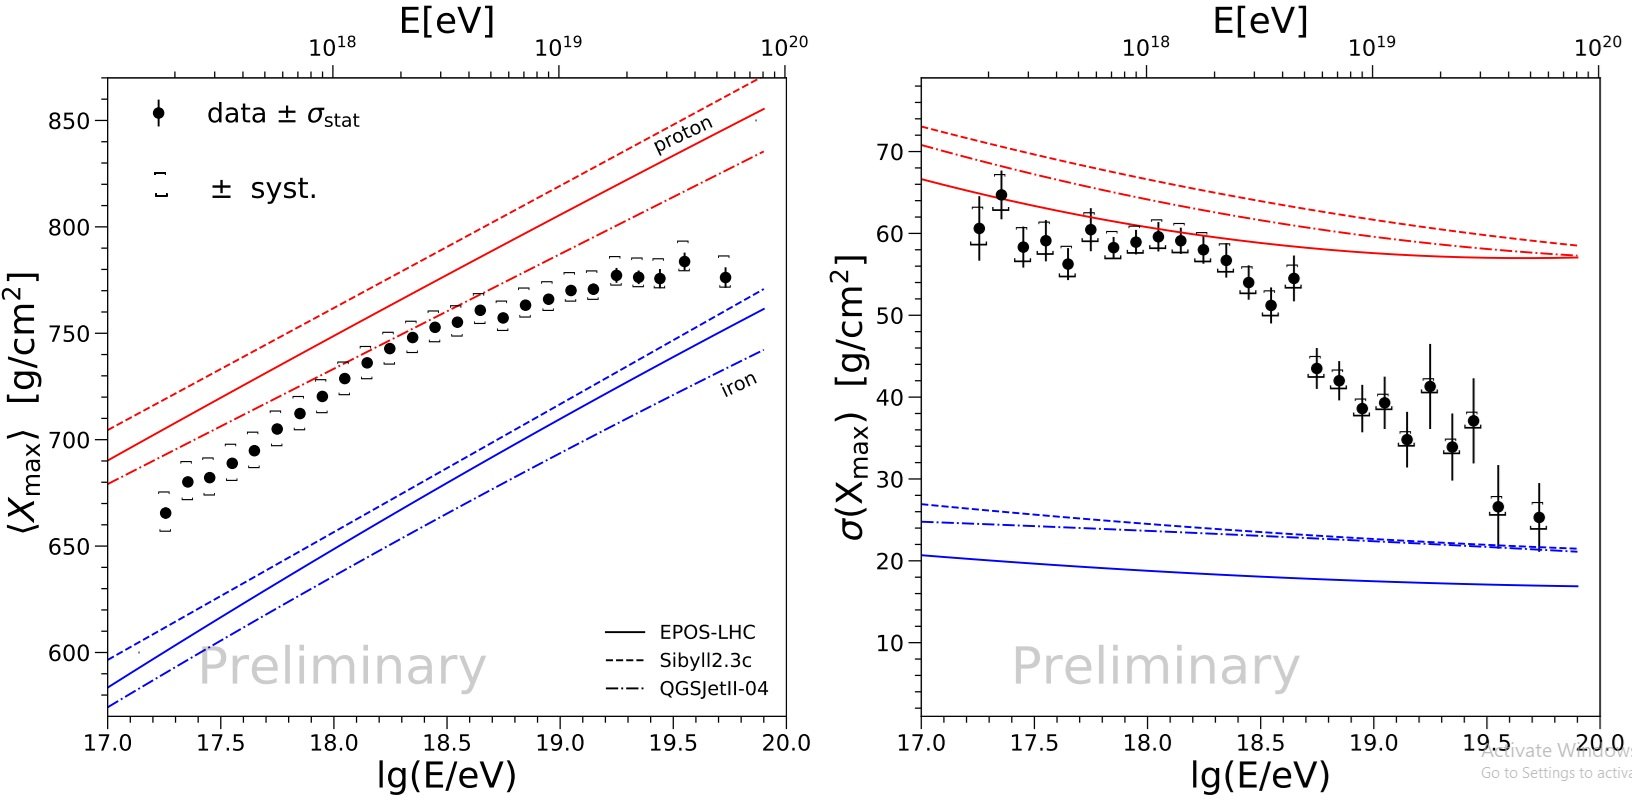
\includegraphics[width=1\textwidth]{capitulos/imagenes_capitulos/cap5/x_max.jpg}
	\caption{Evolución del valor medio de $X_{\text{max}}$ (izquierda) y sus fluctuaciones (derecha) en función de la energía primaria, medido por el Observatorio Pierre Auger. Se observan las curvas teóricas de los modelos hadrónicos acotando el comportamiento entre protón (líneas rojas superiores) y hierro (líneas azules inferiores). Se ve también la dependencia lineal que hay entre el $X_{max}$ y el logaritmo de la energia del primario. Extraído de \cite{yushkov2019mass}.}
	\label{fig:auger_xmax}
\end{figure}

Para comprender por qué esta diferencia en la profundidad del máximo impacta directamente sobre la amplitud de asimetría $A_{1}$ medida en superficie, es necesario analizar la dinámica del desarrollo longitudinal y su proyección topológica sobre el arreglo.

\begin{figure}[H]
	\centering
	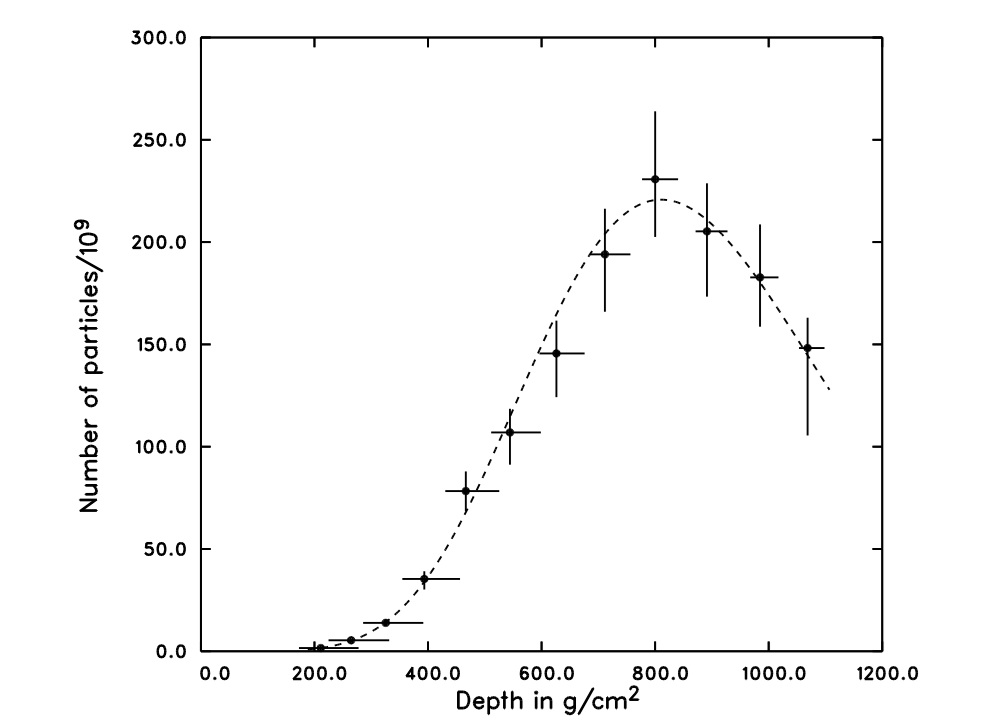
\includegraphics[width=1\textwidth]{capitulos/imagenes_capitulos/cap5/ammount_xmax.jpg}
	\caption{El gráfico corresponde al evento de mayor energía detectado por el experimento Fly's Eye ($E \approx 3.2 \times 10^{20}$ eV) extraído de \cite{FlysEye1995}. Se observa claramente la fase de multiplicación hasta alcanzar la profundidad del máximo, seguida de la atenuación de la cascada. La distancia recorrida de atmosfera hasta llegar al máximo es lo que se denomina $X_{max}$.}
	\label{fig:longitudinal_profile}
\end{figure}

Como se ve en la Figura \ref{fig:longitudinal_profile} a medida que la lluvia penetra en la atmósfera, experimenta una fase de multiplicación en avalancha hasta alcanzar la profundidad del máximo, $X_{max}$. Superado este umbral, la energía media de las partículas secundarias cae por debajo de la energía crítica para seguir alimentando la creación de nuevas partículas, momento en el cual los procesos de pérdida por ionización y el decaimiento dominan sobre la sección eficaz de interacción, forzando a la cascada a entrar en su fase de atenuación.

Dado que el UMD es un detector subterráneo, ciego a la componente electromagnética, la asimetría registrada debe depender estrictamente del historial de producción y transporte de la componente muónica. Los muones se originan principalmente a partir del decaimiento de mesones cargados (piones y kaones, ej. $\pi^{\pm} \rightarrow \mu^{\pm} + \nu_{\mu}$). La tasa de producción de estas partículas sigue de cerca el perfil longitudinal del cascada hadrónica y alcanza su propio máximo, denominado $X_{max}^{\mu}$, a una profundidad muy similar al $X_{max}$ \cite{Cazon2012}.

La modulación azimutal remanente en esta componente muónica está gobernada  fundamentalmente por un efecto de proyección geométrica acoplado a la divergencia angular de las partículas. Sea $D$ la distancia que recorren las partículas, medida a lo largo del eje de la lluvia, desde la región de máxima producción muónica ($X_{max}^{\mu}$) hasta el centro del arreglo de detectores en el suelo. Al incidir una cascada inclinada con ángulo cenital $\theta$, la porción del frente de partículas que impacta en la región tardía debe recorrer una distancia geométrica adicional $\Delta d$ respecto a las partículas que impactan en la región temprana, para un mismo radio $r$ en el plano de la lluvia.

Dado que la densidad de partículas provenientes de un haz colimado decae radialmente como la divergencia espacial  $\propto 1/d^2$ \cite{Cazon2012}, la magnitud de la asimetría temprano-tardía producida por este efecto depende fuertemente del cociente entre la diferencia de camino y la distancia total de propagación $\Delta d / D$.

Cuando una lluvia inducida por un núcleo de Hierro impacta contra el arreglo, el observador percibe una cascada en un estado longitudinal maduro. Debido a que su $X_{max}$ se encuentra a bajas profundidades atmosféricas (altas altitudes geográficas), la distancia geométrica $D$ desde el punto de producción hasta el suelo es inmensa. En consecuencia, el camino extra $\Delta d$ requerido para alcanzar la región tardía representa una fracción marginal del trayecto total ($\Delta d / D \ll 1$). Ademas tras recorrer decenas de kilómetros, la dispersión cinemática intrínseca y la deflexión geomagnética homogenizan las trayectorias de los muones, mitigando las diferencias bruscas y resultando en una distribución azimutalmente uniforme, lo que se traduce en un valor de $A_1$ comparativamente bajo.

En contraste, los primarios livianos (Protones) penetran profundamente en la atmósfera, situando su $X_{max}$ mucho más próximo a la superficie topográfica. Esta proximidad reduce severamente la distancia $D$, incrementando significativamente el peso relativo de la dispersión espacial ($\Delta d / D$). Para frentes de cascada ubicados cerca del punto de observación, la atenuación longitudinal castigan asimétricamente a la región tardía frente a la región temprana generado un valor de asimetría mayor.

En conclusión, la profundidad de penetración del primario modula la agudeza topológica de la cascada medida en tierra. Las lluvias con un $X_{max}$ profundo (protones o lluvias de mayor energía) exponen al UMD a frentes de partículas más concentrados espacialmente, donde cualquier diferencia de proyección geométrica induce fluctuaciones grandes en las densidades relativas de muones. Este mecanismo fenomenológico consolida a la amplitud de asimetría $A_1$ no solo como un descriptor morfológico de la LDF, sino como un trazador valioso de la evolución longitudinal y, en última instancia, como un instrumento extra para realizar discriminación de la masa $A$ del rayo cósmico primario.

\subsubsection{Contraste fenomenológico con el Detector de Superficie}
\label{subsec:contraste_sd_bradfield}

El comportamiento de la asimetría azimutal ha sido desarrollado en detalle en el trabajo de Bradfield \cite{BradfieldThesis} aplicado a las señales del Detector de Superficie (SD). Es pertinente contextualizar los resultados obtenidos con el UMD frente a dichos estudios para evidenciar la naturaleza divergente de las componentes de la cascada.

Al analizar la dependencia de la asimetría con la evolución longitudinal de la cascada, surge una discrepancia física fundamental. En los análisis realizados sobre el SD, se reporta que la magnitud de la asimetría experimenta un decrecimiento a medida que aumenta la profundidad del máximo ($X_{max}$). Este comportamiento es directamente opuesto a la dinámica observada empíricamente en el UMD en las simulaciones, donde frentes de cascada más profundos (primarios livianos o de mayor energía) inducen una mayor amplitud $A_1$.

Esta aparente contradicción se puede explicar al considerar los regímenes físicos fundamentalmente distintos que dominan la propagación de cada componente atmosférica. La asimetría medida por el SD está gobernada de manera abrumadora por la componente electromagnética ($e^\pm, \gamma$). Como fue formalizado por Dova \textit{et al.} \cite{dova2003}, la asimetría de esta componente surge de la variación azimutal en el espesor atmosférico atravesado. Al propagarse en un régimen de rápida atenuación, la amplitud de la asimetría resulta proporcional al gradiente local de la curva de desarrollo longitudinal de la cascada:

\begin{equation}
	A_{EM} \propto \frac{1}{\rho_{EM}} \frac{\partial \rho_{EM}}{\partial X} \Delta X
	\label{eq:asym_em_taylor}
\end{equation}

Para las cascadas típicas observadas en Auger, el nivel del suelo se encuentra a una profundidad mayor que $X_{max}$, situando a los detectores en la fase de decaimiento de la curva de desarrollo. A medida que $X_{max}$ aumenta y la lluvia penetra más en la atmósfera, el punto de observación se aproxima al máximo de la cascada. En esta región de la curva de Gaisser-Hillas, la pendiente de atenuación es significativamente más suave (el gradiente $\partial \rho_{EM} / \partial X$ tiende a cero). Al desvanecerse este gradiente, la diferencia neta de densidad entre las regiones temprana y tardía inducida por el $\Delta X$ se suprime, lo que provoca el colapso sistemático de la asimetría observada en el SD reportado en \cite{BradfieldThesis}.

En estricto contraste, el UMD registra de manera pura la componente muónica. Tal como fue establecido inicialmente por Billoir \cite{GAP2000_017} y expandido en los modelos de Ave \textit{et al.} \cite{ave2017}, los muones de alta energía poseen una propagación cuasi-rectilínea y su distribución responde a la distancia geométrica al punto de producción en lugar del espesor atmosférico. Consecuentemente, su modulación azimutal es un efecto cinemático derivado de la divergencia del flujo de partículas, donde la densidad en el suelo decae con la inversa del cuadrado de la distancia ($\rho_\mu \propto 1/d^2$). 

Para una lluvia cuyo centro se produce a una distancia $D$ sobre el eje, un detector ubicado a un radio $r$ en el suelo se encuentra a una distancia efectiva $d \approx D - r \sin\theta \cos\phi$ respecto a la fuente, debido a la inclinación del frente. Aplicando una expansión de Taylor de primer orden (válida para $r \ll D$), la densidad angular resulta:

\begin{equation}
	\rho(\phi) \propto \frac{1}{(D - r \sin\theta \cos\phi)^2} \approx \frac{1}{D^2} \left( 1 + 2 \frac{r \sin\theta}{D} \cos\phi \right)
\end{equation}

Comparando esta expresión con la parametrización armónica estándar $\rho(\phi) = \rho_0 (1 + A_1 \cos\phi)$, se deriva directamente que la asimetría muónica depende de la inversa de la distancia de producción:

\begin{equation}
	A_{\mu} \approx 2 \frac{r \sin\theta}{D}
	\label{eq:asym_mu_cinematica}
\end{equation}

Un evento con un $X_{max}$ profundo implica que el rayo cósmico ha penetrado más en la atmósfera, situando el punto de producción muónica significativamente más cerca de los detectores. Esta proximidad reduce drásticamente el denominador $D$ en la Ec. \ref{eq:asym_mu_cinematica}. Al achicarse la distancia total de propagación, las diferencias espaciales relativas se magnifican, justificando el marcado incremento de la amplitud $A_1$ medido en el UMD para lluvias más penetrantes.

Finalmente, es crucial rediscutir la interpretación fenomenológica respecto a la composición primaria propuesta para el SD. Bradfield atribuye la menor asimetría del hierro respecto al protón, a igualdad de $X_{max}$, a su 'contenido adicional de muones'. Físicamente, la normalización absoluta de la componente muónica no altera la modulación relativa de su propia distribución. El origen de este corrimiento reside en el principio de superposición que ya se discutió en la sección \ref{subsec:interpretacion_fisica}. El SD mide una señal promediada ponderada por fracciones ($A^{SD} \approx f_{EM} A_{EM} + f_{\mu} A_{\mu}$). Como las lluvias inducidas por primarios pesados poseen una fracción de señal muónica ($f_{\mu}$) intrínsecamente mayor, el promedio del SD otorga más peso estadístico al término menos asimétrico ($A_{\mu}$), diluyendo la asimetría global observada. 

Esta caracterización cinemática demuestra que el SD constituye un observable de difícil interpretación para estudios de composición a través de la asimetría, debido a la supresión de su gradiente longitudinal cerca del máximo. En contrapartida, el UMD aísla un mecanismo estrictamente proyectivo regido por $1/D$, consolidándose como un instrumento robusto y físicamente transparente para estudiar el desarrollo de la lluvia.

\newpage
	% !TEX root = ../main.tex

\section{Dinámica Radial y Desacople Instrumental en el Arreglo \textit{Infill}}
\label{cap:infill}

Habiendo validado la fenomenología de la asimetría azimutal en el entorno geométricamente controlado del Anillo Denso, es imperativo extender el análisis a la topología real del arreglo de detectores. A diferencia de un muestreo isorradial, el arreglo \textit{Infill} expone a las estaciones de superficie y a los módulos subterráneos a un espectro continuo de distancias al eje de la lluvia. En este capítulo se aborda cómo la dinámica de la cascada y la resolución instrumental modulan el observable $A_1$, marcando la transición desde un régimen de dominancia cinemática hacia uno de atenuación longitudinal.

\subsection{Evolución de la asimetría con la distancia al eje}
\label{sec:evolucion_radial}

La modulación azimutal de la densidad de muones en superficie no es un parámetro espacialmente invariante. La aproximación de un único valor global de asimetría para toda la cascada resulta insuficiente al analizar datos experimentales, ya que el frente de partículas presenta gradientes de densidad severos. En el Capítulo \ref{sec:cap_anillo_denso}, la fijación del radio a $r = 450$~m permitió aislar el término armónico de la Función de Distribución Lateral (LDF). Sin embargo, al incorporar el arreglo \textit{Infill} en su totalidad, la amplitud $A_1$ debe ser tratada formalmente como una función explícita de la distancia al eje, $A_1(r)$. Esta dependencia radial es la manifestación directa de la variación en las poblaciones muónicas muestreadas por los detectores: partículas producidas en diferentes altitudes geográficas y con diferentes momentos transversales ($p_T$) dominan distintas regiones del plano topográfico.

\subsection{El Cruce de Asimetría (\textit{Crossover})}
\label{sec:crossover}

Como se estableció teóricamente, la asimetría neta surge de la competencia entre la atenuación atmosférica y el efecto de proyección geométrica acoplado a la divergencia angular. El peso relativo de ambos mecanismos evoluciona de manera drástica con la distancia al núcleo $r$, generando un punto de transición o \textit{crossover} topológico.

En la región del \textit{near-core} ($r < 200$~m), la densidad de partículas está gobernada por la divergencia cinemática de muones producidos con alto $p_T$. Estas partículas conservan trayectorias con gran inclinación respecto al eje de la lluvia, maximizando el factor de asimetría espacial ($\Delta d / D$). La exigencia de recorrer una distancia adicional para impactar en la zona temprana del detector induce un déficit relativo de señal en $\phi = 0^\circ$ frente a la acumulación en $\phi = \pm 180^\circ$. En consecuencia, el efecto geométrico domina por completo la morfología del frente a cortas distancias, forzando a la amplitud a tomar valores negativos o nulos ($A_1 \le 0$).

Por el contrario, al transitar hacia el \textit{far-core} ($r > 400$~m), la fenomenología se invierte. Las partículas detectadas a grandes radios laterales provienen predominantemente de las primeras generaciones hadrónicas de la cascada. Al originarse a mayor altitud, la distancia de propagación $D$ es inmensa, lo que minimiza el peso relativo de la dispersión espacial ($\Delta d / D \ll 1$). En este régimen, el vasto espesor atmosférico atravesado exponencialmente magnifica las pérdidas por decaimiento y absorción. La atenuación longitudinal recupera el dominio del sistema, castigando severamente a los muones tardíos y restaurando la asimetría positiva característica ($A_1 > 0$).

% [AQUÍ DEBERÍAS INSERTAR TU GRÁFICO DE BINES RADIALES MOSTRANDO EL CROSSOVER]

\subsection{La Singularidad del Núcleo}
\label{sec:singularidad_nucleo}

A pesar de que el modelo cinemático describe satisfactoriamente la asimetría negativa a bajas distancias, el estudio empírico para $r \lesssim 100$~m presenta un desafío metodológico insoslayable. En la vecindad inmediata del impacto, la coherencia de la fase azimutal se degrada abruptamente, destruyendo el ajuste armónico. 

Esta pérdida de señal no obedece a una isotropización intrínseca de la lluvia, sino a una singularidad geométrica fuertemente acoplada a la resolución instrumental. La definición de la fase $\phi$ depende del vector desplazamiento entre la posición reconstruida del núcleo y la estación detectora. En el \textit{Infill}, la incertidumbre espacial intrínseca de la reconstrucción ($\sigma_{core}$) oscila entre $20$~m y $40$~m. 

Para distancias laterales grandes ($r \gg \sigma_{core}$), las fluctuaciones estadísticas del núcleo inducen variaciones angulares despreciables ($\Delta \phi \approx \sigma_{core} / r \ll 1$). Sin embargo, cuando el detector se ubica dentro o en el borde del radio de incerteza geométrica ($r \sim \sigma_{core}$), la relación matemática diverge. Una variación marginal en la estimación del núcleo puede invertir el vector desplazamiento, generando un salto espurio de $\pm 180^\circ$ en la fase asignada a esa estación. Para garantizar la fidelidad del parámetro $A_1$, aislando la física de la cascada de las limitaciones de resolución topográfica, el análisis de los eventos reconstruidos exige la imposición de un corte fiducial radial, excluyendo sistemáticamente las estaciones a $r < 100$~m.

\subsection{Fallas en el SD: Inversiones espurias de asimetría}
\label{subsec:fallas_sd}

\subsection{Análisis del \textit{Survival Ratio} y validación del UMD}
\label{subsec:survival_ratio}
% N_\mu^{\mathrm{UMD}} / N_\mu^{\mathrm{SD}} y contaminación sub-GeV.

\newpage
	% !TEX root = ../main.tex

\section{Análisis de Asimetría en Datos Experimentales}
\label{sec:datos_reales}

\subsection{Selección de datos experimentales del \textit{Infill}}
\label{subsec:seleccion_datos}

\subsection{Extracción de la asimetría azimutal en datos reales}
\label{subsec:extraccion_asimetria}

\subsection{Comparación Datos vs. MC y composición de masa media}
\label{subsec:comparacion_mc_datos}

\newpage
	% !TEX root = ../main.tex

\section{Conclusiones}
\label{sec:conclusiones}

\subsection{Síntesis de resultados}
\label{subsec:sintesis}

\subsection{Perspectivas futuras}
\label{subsec:perspectivas}

\newpage
	
	% ==========================================
	% BIBLIOGRAFÍA
	% ==========================================
	\newpage
	\printbibliography[heading=bibintoc, title={Referencias}]
	
\end{document}\documentclass[spanish,a4paper,11pt]{article}